

\chapter{Evolution of smartphone features}
\label{ape:gsmarena-n95-s7}

Regarding the upgrades throughout the years we can see here that in 10 years the processors are almost 10 times faster in each core, the memory capacity is 25 times bigger now, and  the communication technologies increased the number of network bands and the bandwidth.
It is interesting to notice that in 2006 we already have a smartphone with WLAN, 3G, Bluetooth, infrared, GPS and radio technologies into a single board.

\begin{longtable}{llp{0.3\linewidth}p{0.3\linewidth}}
\caption{Communication technologies available on smartphones with 10 years announcement difference: Nokia N95 (2006) and Samsung Galaxy S7 (2016). Source: Adapted from \cite{GSMARENA2016-n95-s7}} \\ \hline
         &               & Nokia N95                                                   & Samsung Galaxy S7                                                                                                                                                                                                  \\ \hline \endhead
         
LAUNCH   & Announced     & 2006, September. Released 2007, March                        & 2016, February                                                                                                                                                                                              \\
         & Status        & Discontinued                                                 & Available. Released 2016, March                                                                                                                                                                             \\ \hline
         
PLATFORM & CPU           & 332 MHz Dual ARM 11                                          & Dual-core 2.15 GHz Kryo \& Dual-core 1.6 GHz Kryo or Quad-core 2.3 GHz Mongoose + Quad-core 1.6 GHz Cortex-A53                                                                                                                                                           \\ \hline
MEMORY   & Card slot     & microSD, up to 8 GB (dedicated slot), 128 MB included        & microSD, up to 200 GB (dedicated slot)                                                                                                                                                \\
         &               &                                                              & microSD, up to 200 GB                                                                                                                                                   \\
         & Internal      & 160 MB, 64 MB RAM                                            & 32/64 GB, 4 GB RAM                                                                                                                                                                                          \\ \hline
NETWORK  & Technology    & GSM / HSPA                                                   & GSM / HSPA / LTE                                                                                                                                                                                            \\
         & 2G bands      & GSM 850 / 900 / 1800 / 1900                                  & GSM 850 / 900 / 1800 / 1900                            \\
         & 3G Network    & HSDPA 2100                                                   & HSDPA 850 / 900 / 1700(AWS) / 1900 / 2100 - G930F                                                                                                                                                           \\
         &               & HSDPA 850 / 1900                          & TD-SCDMA                                                                                                                                                                                                    \\
         & 4G Network    &                                                              & LTE band 1(2100), 2(1900), 3(1800), 4(1700/2100), 5(850), 7(2600), 8(900), 12(700), 13(700), 17(700), 18(800), 19(800), 20(800), 25(1900), 26(850), 28(700), 38(2600), 39(1900), 40(2300), 41(2500) - G930F \\
         & Speed         & HSPA                                                         & HSPA 42.2/5.76 Mbps, LTE Cat9 450/50 Mbps                                                                                                                                                                   \\
         & GPRS          & Class 10                                                     & Yes                                                                                                                                                                                                         \\
         & EDGE          & Class 32, 296 kbps; DTM Class 11, 177 kbps                   & Yes                                                                                                                                                                                                         \\ \hline
COMMS    & WLAN          & Wi-Fi 802.11 b/g, UPnP technology                            & Wi-Fi 802.11 a/b/g/n/ac, dual-band, Wi-Fi Direct, hotspot                                                                                                                                                   \\
         & Bluetooth     & v2.0, A2DP                                                   & v4.2, A2DP, LE, aptX                                                                                                                                                                                        \\
         & GPS           & Yes, with A-GPS; Nokia Maps                                  & Yes, with A-GPS, GLONASS, BDS                                                                                                                                                                               \\
         & NFC           & No                                                           & Yes                                                                                                                                                                                                         \\
         & Infrared port & Yes                                                          & No                                                                                                                                                                                                          \\
         & Radio         & Stereo FM radio                                              & No                                                                                                                                                                                                          \\
         & USB           & miniUSB v2.0                                                 & microUSB v2.0, USB Host                                                                                                                                                                                     \\ \hline
\label{tab:gsmarena-n95-s7}
\end{longtable}





\chapter{Available sensors within the Android system}
\label{ape:android-sensors}

Here we have some sensors available for mobile devices, being the base sensors the ones that are related to physical sensors while the others are composite sensors that use values from the base sensors or merge two or more sensors.

% \begin{table}[]
% \centering

\begin{longtable}{@{}llllll@{}}
\caption{Definition of available sensors for Android system. Source: \cite{Android2016sensorssource,Android2016sensortypes}} \\ \hline
Sensor type                   & ID & \begin{tabular}[c]
{@{}l@{}}Reporting\\ mode\end{tabular} & \begin{tabular}[c]
{@{}l@{}}\# of \\ values\end{tabular} & \begin{tabular}[c]
{@{}l@{}}Composite\\ category\end{tabular} & \begin{tabular}[c]
{@{}l@{}}Low\\ power\end{tabular} \\ \hline \endhead
ACCELEROMETER                 & 1  & continuous   & 3         & (base sensor)    &           \\
GEOMAGNETIC\_FIELD            & 2  & continuous   & 3         & (base sensor)    &           \\
ORIENTATION                   & 3  & continuous   & 3         & attitude         &           \\
GYROSCOPE                     & 4  & continuous   & 3         & (base sensor)    &           \\
LIGHT                         & 5  & on-change    & 1         & (base sensor)    &           \\
PRESSURE                      & 6  & continuous   & 1         & (base sensor)    &           \\
TEMPERATURE                   & 7  &              & 1         &                  &           \\
PROXIMITY                     & 8  & on-change    & 1         & (base sensor)    &           \\
GRAVITY                       & 9  & continuous   & 3         & attitude         &           \\
LINEAR\_ACCELERATION          & 10 & continuous   & 3         & activity         &           \\
ROTATION\_VECTOR              & 11 & continuous   & 4         & attitude         &           \\
RELATIVE\_HUMIDITY            & 12 & on-change    & 1         & (base sensor)    &           \\
AMBIENT\_TEMPERATURE          & 13 & on-change    & 1         & (base sensor)    &           \\
MAGNETIC\_FIELD\_UNCALIBRATED & 14 & continuous   & 6         & uncalibrated     &           \\
GAME\_ROTATION\_VECTOR        & 15 & continuous   & 3         & attitude         &           \\
GYROSCOPE\_UNCALIBRATED       & 16 & continuous   & 6         & uncalibrated     &           \\
SIGNIFICANT\_MOTION           & 17 & one-shot     & 1         & activity         & yes       \\
STEP\_DETECTOR                & 18 & special      & 1         & activity         & yes       \\
STEP\_COUNTER                 & 19 & on-change    & 1         & activity         & yes       \\
GEOMAGNETIC\_ROTATION\_VECTOR & 20 & continuous   & 4         & attitude         & yes       \\
HEART\_RATE                   & 21 & on-change    & 1         & (base sensor)    &           \\
TILT\_DETECTOR                & 22 & special      & 1         & activity         & yes       \\
WAKE\_GESTURE                 & 23 & one-shot     & 1         & interaction      & yes       \\
GLANCE\_GESTURE               & 24 & one-shot     & 1         & interaction      & yes       \\
PICK\_UP\_GESTURE             & 25 & one-shot     & 1         & interaction      & yes       \\
WRIST\_TILT\_GESTURE          & 26 & special      & 1         &                  & yes       \\ \hline
\label{tab:android-sensors}
\end{longtable}




\chapter{Devices used during research}
\label{ape:gsmarena-lg-s3-z3}

The mobile devices used during this research were the LG D686 G Pro Dual Lite, Samsung GT-I9300 Galaxy SIII, and Sony Xperia D8533 (and D8503) Z3 Compact.
Their technical specifications are presented on the Table \ref{tab:gsmarena-lg-s3-z3}. 

\begin{longtable}{llp{0.2\linewidth}p{0.2\linewidth}p{0.2\linewidth}}
	\caption{Technical specifications of the mobile devices used during this research: D686, S3, and Z3. Source: Adapted from \cite{GSMARENA2017-lg-s3-z3}} \\ \hline
		&               & LG D686 G Pro Lite Dual                              & Samsung GT-I9300 Galaxy SIII                                                                  & Sony D8533 (and D8503) Xperia Z3 Compact                                                                                         \\ \hline \endhead
		NETWORK  & Technology    & GSM / HSPA                                      & GSM / HSPA                                                                                  & GSM / HSPA / LTE                                                                                               \\
		& 2G bands      & GSM 850 / 900 / 1800 / 1900 - SIM 1 \& SIM 2    & GSM 850 / 900 / 1800 / 1900                                                                 & GSM 850 / 900 / 1800 / 1900                                                                                    \\
		& 3G Network    & HSDPA 850 / 900 / 1900 / 2100                   & HSDPA 850 / 900 / 1900 / 2100                                                               & HSDPA 850 / 900 / 1700 / 1900 / 2100 - D5803                                                                   \\
		&               &                                                 &                                                                                             & HSDPA 850 / 900 / 1900 / 2100 - D5833                                                                          \\
		& 4G Network    &                                                 &                                                                                             & LTE band 1(2100), 2(1900), 3(1800), 4(1700/2100), 5(850), 7(2600), 8(900), 13(700), 17(700), 20(800) - D5803   \\
		&               &                                                 &                                                                                             & LTE band 1(2100), 3(1800), 5(850), 7(2600), 8(900), 28(700), 40(2300) - D5833                                  \\
		& Speed         & HSPA 7.2/5.76 Mbps                              & HSPA 21.1/5.76 Mbps                                                                         & HSPA 42.2/5.76 Mbps, LTE Cat4 150/50 Mbps                                                                      \\
		& GPRS          & Class 12                                        & Class 12                                                                                    & Up to 107 kbps                                                                                                 \\
		& EDGE          & Class 12                                        & Class 12                                                                                    & Up to 296 kbps                                                                                                 \\ \hline
		LAUNCH   & Announced     & 2013, October                                   & 2012, May                                                                                   & 2014, September                                                                                                \\
		& Status        & Available. Released 2013, November              & Available. Released 2012, May                                                               & Available. Released 2014, September                                                                            \\ \hline
		PLATFORM & OS            & Android OS, v4.1.2 (Jelly Bean)                 & Android OS, v4.0.4 (Ice Cream Sandwich), 4.3 (Jelly Bean)                                   & Android OS, v4.4.4 (KitKat), upgradable to v6.0 (Marshmallow)                                                  \\
		& Chipset       & Mediatek MT6577                                 & Exynos 4412 Quad                                                                            & Qualcomm MSM8974AC Snapdragon 801                                                                              \\
		& CPU           & Dual-core 1.0 GHz Cortex-A9                     & Quad-core 1.4 GHz Cortex-A9                                                                 & Quad-core 2.5 GHz Krait 400                                                                                    \\
		& GPU           & PowerVR SGX531                                  & Mali-400MP4                                                                                 & Adreno 330                                                                                                     \\ \hline
		MEMORY   & Card slot     & microSD, up to 32 GB (dedicated slot)           & microSD, up to 64 GB (dedicated slot)                                                       & microSD, up to 256 GB (dedicated slot)                                                                         \\
		& Internal      & 8 GB, 1 GB RAM                                  & 16/32/64 GB, 1 GB RAM                                                                       & 16 GB, 2 GB RAM                                                                                                \\ \hline
		COMMS    & WLAN          & Wi-Fi 802.11 b/g/n, Wi-Fi Direct, DLNA, hotspot & Wi-Fi 802.11 a/b/g/n, dual-band, Wi-Fi Direct, DLNA, hotspot                                & Wi-Fi 802.11 a/b/g/n/ac, dual-band, Wi-Fi Direct, DLNA, hotspot                                                \\
		& Bluetooth     & v3.0, A2DP                                      & v4.0, A2DP, EDR, aptX                                                                       & v4.0, A2DP, LE, aptX                                                                                           \\
		& GPS           & Yes, with A-GPS                                 & Yes, with A-GPS, GLONASS                                                                    & Yes, with A-GPS, GLONASS                                                                                       \\
		& NFC           &                                                 & Yes                                                                                         & Yes                                                                                                            \\
		& Infrared port & Yes                                             & No                                                                                          & No                                                                                                             \\
		& Radio         & FM radio                                        & Stereo FM radio, RDS                                                                        & Stereo FM radio, RDS                                                                                           \\
		& USB           & microUSB v2.0                                   & microUSB v2.0 (MHL TV-out), USB Host                                                        & microUSB v2.0 (MHL TV-out), USB Host; magnetic connector                                                       \\ \hline
		FEATURES & Sensors       & Accelerometer, proximity, compass               & Accelerometer, gyro, proximity, compass, barometer                                          & Accelerometer, gyro, proximity, compass, barometer                                                             \\ \hline
		BATTERY  &               & Removable Li-Ion 3140 mAh battery               & Removable Li-Ion 2100 mAh battery                                                           & Non-removable Li-Ion 2600 mAh battery                                                                          \\
		& Stand-by      & Up to 845 h                                     & Up to 590 h (2G) / Up to 790 h (3G)                                                         & Up to 880 h (2G) / Up to 920 h (3G)                                                                            \\
		& Talk time     & Up to 14 h 30 min                               & Up to 21 h 40 min (2G) / Up to 11 h 40 min (3G)                                             & Up to 12 h (2G) / Up to 14 h (3G)                                                                              \\
		& Music play    &                                                 &                                                                                             & Up to 110 h           \\ \hline                                                                                                                                                                                    
\label{tab:gsmarena-lg-s3-z3}
\end{longtable}



Two specific routers were bought in order to be used during the evaluation. 
One router was maintained at USP while the other was situated at UMich.
The technical details about the routers are described at Table \ref{tab:tplink-ac1750}.

\begin{longtable}{lp{0.7\linewidth}}		
\caption{Technical specifications of the TP-Link AC1750 Archer C7 Wireless Dual Band Gigabit Router. Source: Addapted from \cite{TPLINK2017AC1750}} \\ \hline
		HARDWARE FEATURES 		 		 		 		 & \\ 
		Interface 		 		 		 		 & 4 10/100/1000Mbps LAN Ports\\
													 & 1 10/100/1000Mbps WAN Port\\
													 & 2 USB 2.0 Ports \\
		Button 		 		 		 		 & WPS/Reset Button\\
												 & Wireless On/Off Switch \\
												 & Power On/Off Button \\
		External Power Supply 		 		 		 		 & 12VDC / 2A \\
		Dimensions ( W x D x H ) 		 		 		 		 & 9.6x6.4x1.3 in. (243x160.6x32.5mm) \\
		Antenna Type 		 		 		 		 & Three detachable antennas ( RP-SMA) \\ \hline
		WIRELESS FEATURES 		 		 		 		 & \\
		Wireless Standards 		 		 		 		 & IEEE 802.11ac/n/a 5GHz\\
																	 & IEEE 802.11b/g/n 2.4GHz \\
		Frequency 		 		 		 		 & 2.4GHz and 5GHz \\
		Signal Rate 		 		 		 		 		 & 5GHz: Up to 1300Mbps \\ 
		                                                    & 2.4GHz:  Up to 450Mbps \\
%		Reception Sensitivity 		 		 		 		 		 & 5GHz:\\ 
%																				& 11a 6Mbps: -96dBm\\ 
%																				& 11a 54Mbps: -79dBm \\ 
%																				& 11ac HT20: -71dBm \\
%																				& 11ac HT40: -66dBm \\
%																				& 11ac HT80: -63dBm\\
%																				& 2.4GHz: \\
%																				& 11g 54M: -77dBm\\
%																				& 11n HT20: -74dBm \\
%																				& 11n HT40: -72dBm \\
		Transmit Power 		 		 		 		 		 & CE: \\
																		& \textless20dBm(2.4GHz)\\
																		& \textless23dBm(5GHz) \\
																		& FCC:\\
																		& \textless30dBm \\
		Wireless Functions 		 		 		 		 		 & Enable/Disable Wireless Radio, WDS Bridge, WMM, Wireless Statistics \\
		Wireless Security 		 		 		 		 		 & 64/128-bit WEP, WPA / WPA2, WPA-PSK/ WPA2-PSK encryption \\ \hline
		SOFTWARE FEATURES 		 		 		 		 		 & \\
		Quality of Service 		 		 		 		 		 & WMM, Bandwidth Control \\
		WAN Type 		 		 		 		 		 & Dynamic IP/Static IP/PPPoE/PPTP(Dual Access)/L2TP(Dual Access)/BigPond \\
		Management 		 		 		 		 		 & Access Control\\
																	& Local Management\\
																	& Remote Management \\
		DHCP 		 		 		 		 		 & Server, Client, DHCP Client List, Address Reservation \\
		Port Forwarding 		 		 		 		 		 & Virtual Server, Port Triggering, UPnP, DMZ \\
		Dynamic DNS 		 		 		 		 		 & DynDns, Comexe, NO-IP \\
		VPN Pass-Through 		 		 		 		 		 & PPTP, L2TP, IPSec \\
		Access Control 		 		 		 		 		 & Parental Control, Local Management Control, Host List, Access Schedule, Rule Management \\
		Firewall Security 		 		 		 		 		 & DoS, SPI Firewall\\
																		& IP Address Filter/MAC Address Filter/Domain Filter\\
																		& IP and MAC Address Binding \\
		Protocols 		 		 		 		 		 & Supports IPv4 and IPv6 \\
		USB Sharing 		 		 		 		 		 & Support Samba(Storage)/FTP Server/Media Server/Printer Server \\
		Guest Network 		 		 		 		 		 & 2.4GHz guest network x 1 \\
																		& 5GHz guest network x 1 \\ \hline
		OTHERS 		 		 		 		 		 & \\
		Certification 		 		 		 		 		 & CE, FCC, RoHS \\ \hline
		\label{tab:tplink-ac1750}
\end{longtable}

%% ------------------------------------------------------------------------- %%
% \chapter{Emails contacted during the research}
% \label{ape:peoplecontacted}

% \begin{longtable}{lp{0.3\linewidth}p{0.3\linewidth}}
% 	\caption{People and emails contacted during research} \\ \hline
% 	Name & Information & Email    \\ \hline \endhead
% Alfredo Goldman vel Lejbman & Director of the Centro de Competência em Software Livre~(CCSL) at IME-USP & gold@ime.usp.br \\
% Multicast support at RNP & Email defined for asking for information regarding Multicast at RNP site & multicast-info@rnp.br  \\
% Multicast list at RNP & Discussion list about Multicast at RNP & majordomo@rnp.br\\
% Information email at RNP & Email available for asking for informations at RNP & info@rnp.br\\
% Helpdesk at RNP & Email used for the helpdesk at RNP & helpdesk@rt.rnp.br\\
% Lisandro Zambenedetti Granville & Co-Chair of the Network Management Research Group of the Internet Research Task Force & granville@inf.ufrgs.br\\
% José Luiz Ribeiro Filho & Director of Services and Solutions Board at RNP & jose.luiz@rnp.br\\
% Antônio Carlos Fernandes Nunes & Adjunct Director of Solutions Management Adjunct Board at RNP & antonio.nunes@rnp.br \\
% NOC - RNP & Network Operations Center contact at RNP & noc@rnp.br\\
% Fábio Rodrigues Ribeiro & Operations Analist at Operations Management of Network Engineering Management at RNP & fabio.ribeiro@rnp.br\\
% Edson Lima Monteiro (aka Boni) & Manager of the Backbone of USP and member of Seção Técnica de Configuração - Divisão de Comunicações - CCE - USP & boni@usp.br\\
% Luiz Eduardo Silva dos Santos & Departamento de Tecnologia da Informação - DTI - USP & lesantos@usp.br\\

% Henrique Cabral de Souza Rodrigues & Técnico em Informática - SI - IME - USP &hcabral@ime.usp.br \\
% & & admin@ime.usp.br\\
% Valter Pereira & & valter.pereira@pop-sp.rnp.br\\
% Wagner Pereira & & wagner.pereira@pop-sp.rnp.br\\
% Rogerio Herrera Mendonça & & rogerio.herrera@pop-sp.rnp.br\\
% Rogerio Herrera & & rogerio@pop-sp.rnp.br\\
% Andre Lopes da Silva & & alopes@ime.usp.br\\
% & & operacao@pop-sp.rnp.br\\
% Roy Hockett & Network Architect, ITS Communications Systems and Data Centers - University of Michigan & royboy@umich.edu\\
% ITSCommna & & itscommna@umich.edu\\

% & & decastro@usp.br\\
% Michael Stanton - RNP && michael@rnp.br\\
% & & noc@redclara.net\\
% & & noc@rnp.br\\
% & & neg@redclara.net\\
% & & rt@eecs.umich.ed\\
% Marco Antonio M. Teixeira & Diretoria Adjunta de Engenharia de Redes e Operações RNP – Rede Nacional de Ensino e Pesquisa & marco.teixeira@rnp.br\\

% William Alexandre Miura Gnann & & gnann@ime.usp.br\\
% Alex Moura & & alex.moura@rnp.br\\
 
% & & pop@pop-sp.rnp.br \\
% & & aluizio.hazin@rnp.br\\
 
% Brian Pullin & & bpullin@grnoc.iu.edu\\
% Brady Farver & & bfarver@umich.edu\\

% Guilherme Ladvocat & GO - Gerência de Operações - DAERO - Diretoria Adjunta de Engenharia de Redes e Operações - RNP - Rede Nacional de Ensino e Pesquisa &  guilherme.ladvocat@rnp.br\\

% Nathan Miller & Indiana University GlobalNOC - Internet2 Network Engineer & ndm2@globalnoc.iu.edu\\
% Christian O'Flaherty & Regional Development - Internet Society  & oflaherty@isoc.org\\
% Iara Machado & & iara@rnp.br\\
% Alex Soares de Moura & & alex@rnp.br\\

% Guillermo Cicileo & & guillermo@lacnic.net\\

%  Eric Boyd & &  eboyd@internet2.edu\\
 
% 		\label{tab:emailscontacted}
% \end{longtable}

% ------------------------------------------------------------------------- %%
 \chapter{Applications created during the research}
 \label{ape:applications}

\input chapterApplications


\chapter{Conference papers published about this research project}
\label{ape:papers}


%% ------------------------------------------------------------------------- %%
\section{SBCM 2013 - FFT benchmark on Android devices: Java versus JNI}
\label{ape:papersbcm2013}

\subsection*{Paper details}

Title: \textit{FFT benchmark on Android devices: Java versus JNI}

Authors: Antonio Deusany de Carvalho Junior, Max Rosan, André Bianchi, Marcelo Queiroz

\subsection*{Conference details}

Title: 14o Simpósio Brasileiro de Computação Musical~(SBCM)

Venue: Escola de Música de Brasília~(EMB), Brasília, DF, Brazil

Dates: October 31 to November 2, 2013

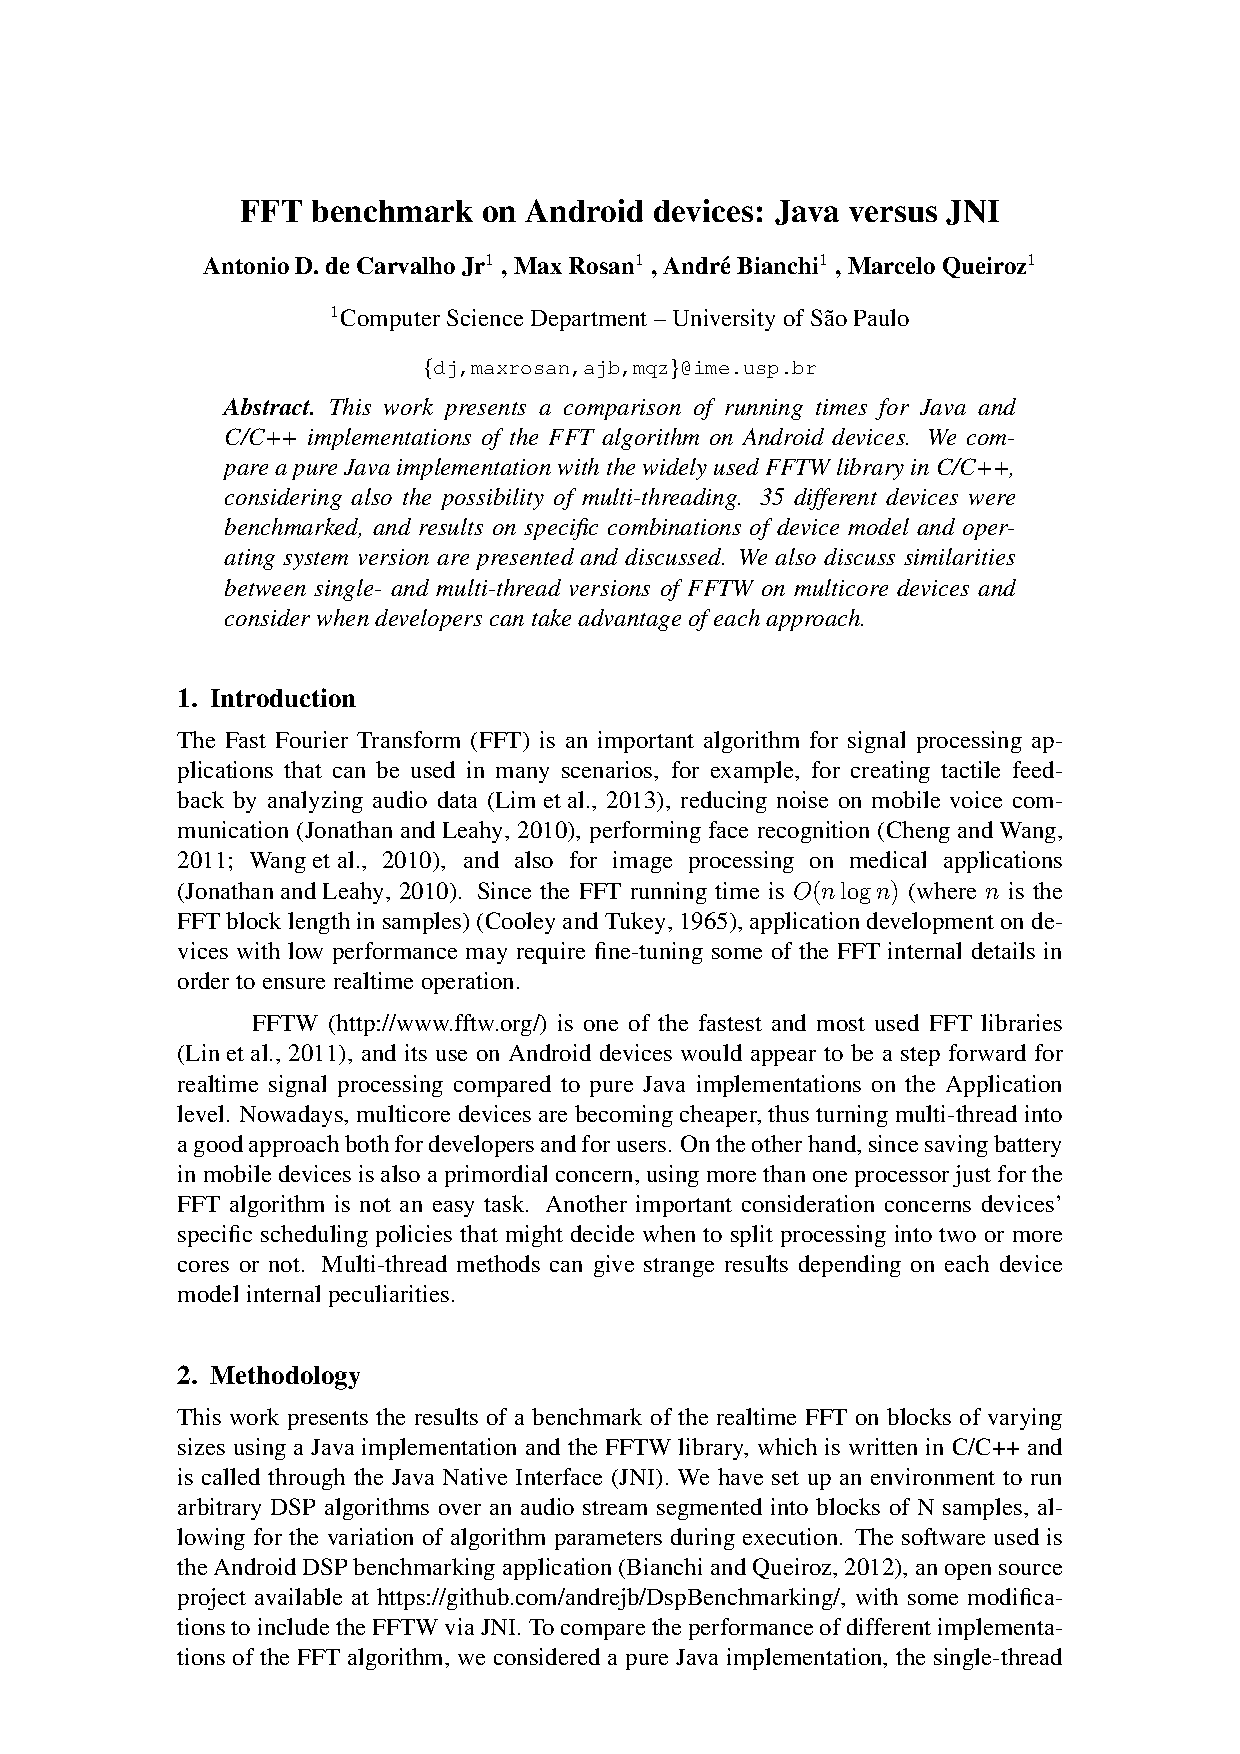
\includepdf[pages=-,frame,scale=0.8,pagecommand={}]{papers/2013-sbcm.pdf}

%% ------------------------------------------------------------------------- %%
\section{ICSC 2013 - Touches on the line: Sharing Csound scores using web server and mobile phones}
\label{ape:papericsc2013}

\subsection*{Paper details}

Title: \textit{Touches on the line: Sharing Csound scores using web server and mobile phones}

Authors: Antonio Deusany de Carvalho Junior

\subsection*{Conference details}

Title: 2nd International CSound Conference~(ICSC)

Venue: Berklee College of Music, Boston, MA, USA

Dates: October 25 to 27, 2013

\subsection*{Remarks}

During the conference, I performed at the Concert \#6 on October 27th with the application running on two mobile devices at the David Friend Recital Hall, Berklee College of Music, Boston, MA, USA~\footnote{\url{http://www.csounds.com/csound-conference-poster-schedule/}}.
This performance happened just before the concert in which performed Jean-Claude Risset, John Chowning, and Richard Boulanger, the masters of Computer Music that I met during this conference.

I also met two important woman for Computer Music during this conference.
Sitting by her side during concerts, I had a brief talk with Marjorie Matthews, the spouse of Max Matthews, the father of Computer Music.
The other woman was Judy Klein, a pianist and professor of electronic music.
We went out for a cup of tea and she exposed me the great history of Computer Music during the 1980's when she was working with the first versions of CSound and waiting the whole night to listen minutes of synthesized sounds.

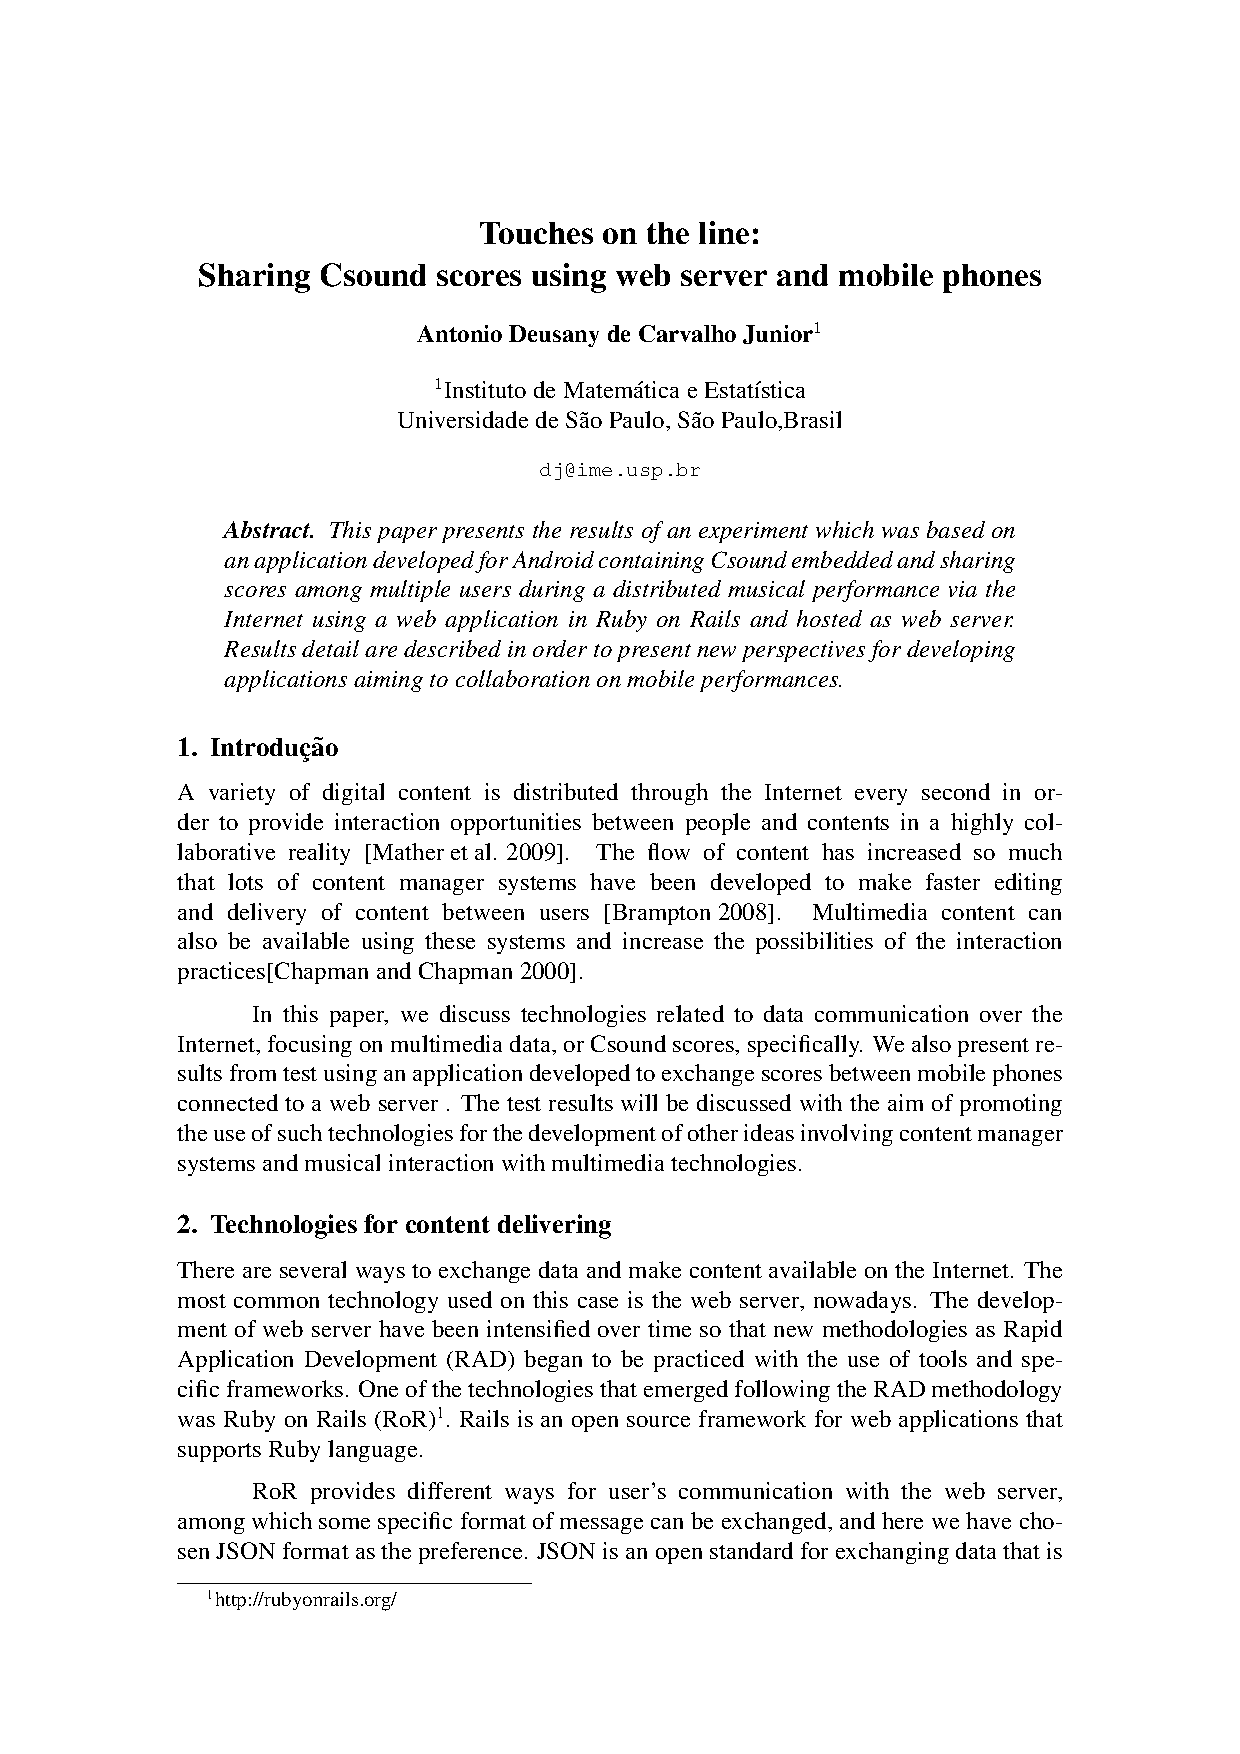
\includepdf[pages=-,frame,scale=0.8,pagecommand={}]{papers/2013-csound.pdf}

%% ------------------------------------------------------------------------- %%
\section{BATS 2014 - Notes on the Elimination of the Mobile Music Audience}
\label{ape:paperbats2014}

\subsection*{Paper details}

Title: \textit{Notes on the Elimination of the Mobile Music Audience}

Authors: André Damião Bandeira, Antonio Deusany de Carvalho Junior

\subsection*{Conference details}

Title: 14th Biennial Arts and Technology Symposium

Venue: Connecticut College, Ammerman Center for Arts and Technology, New London, CT

Dates: February 27, 28 and March 1, 2014


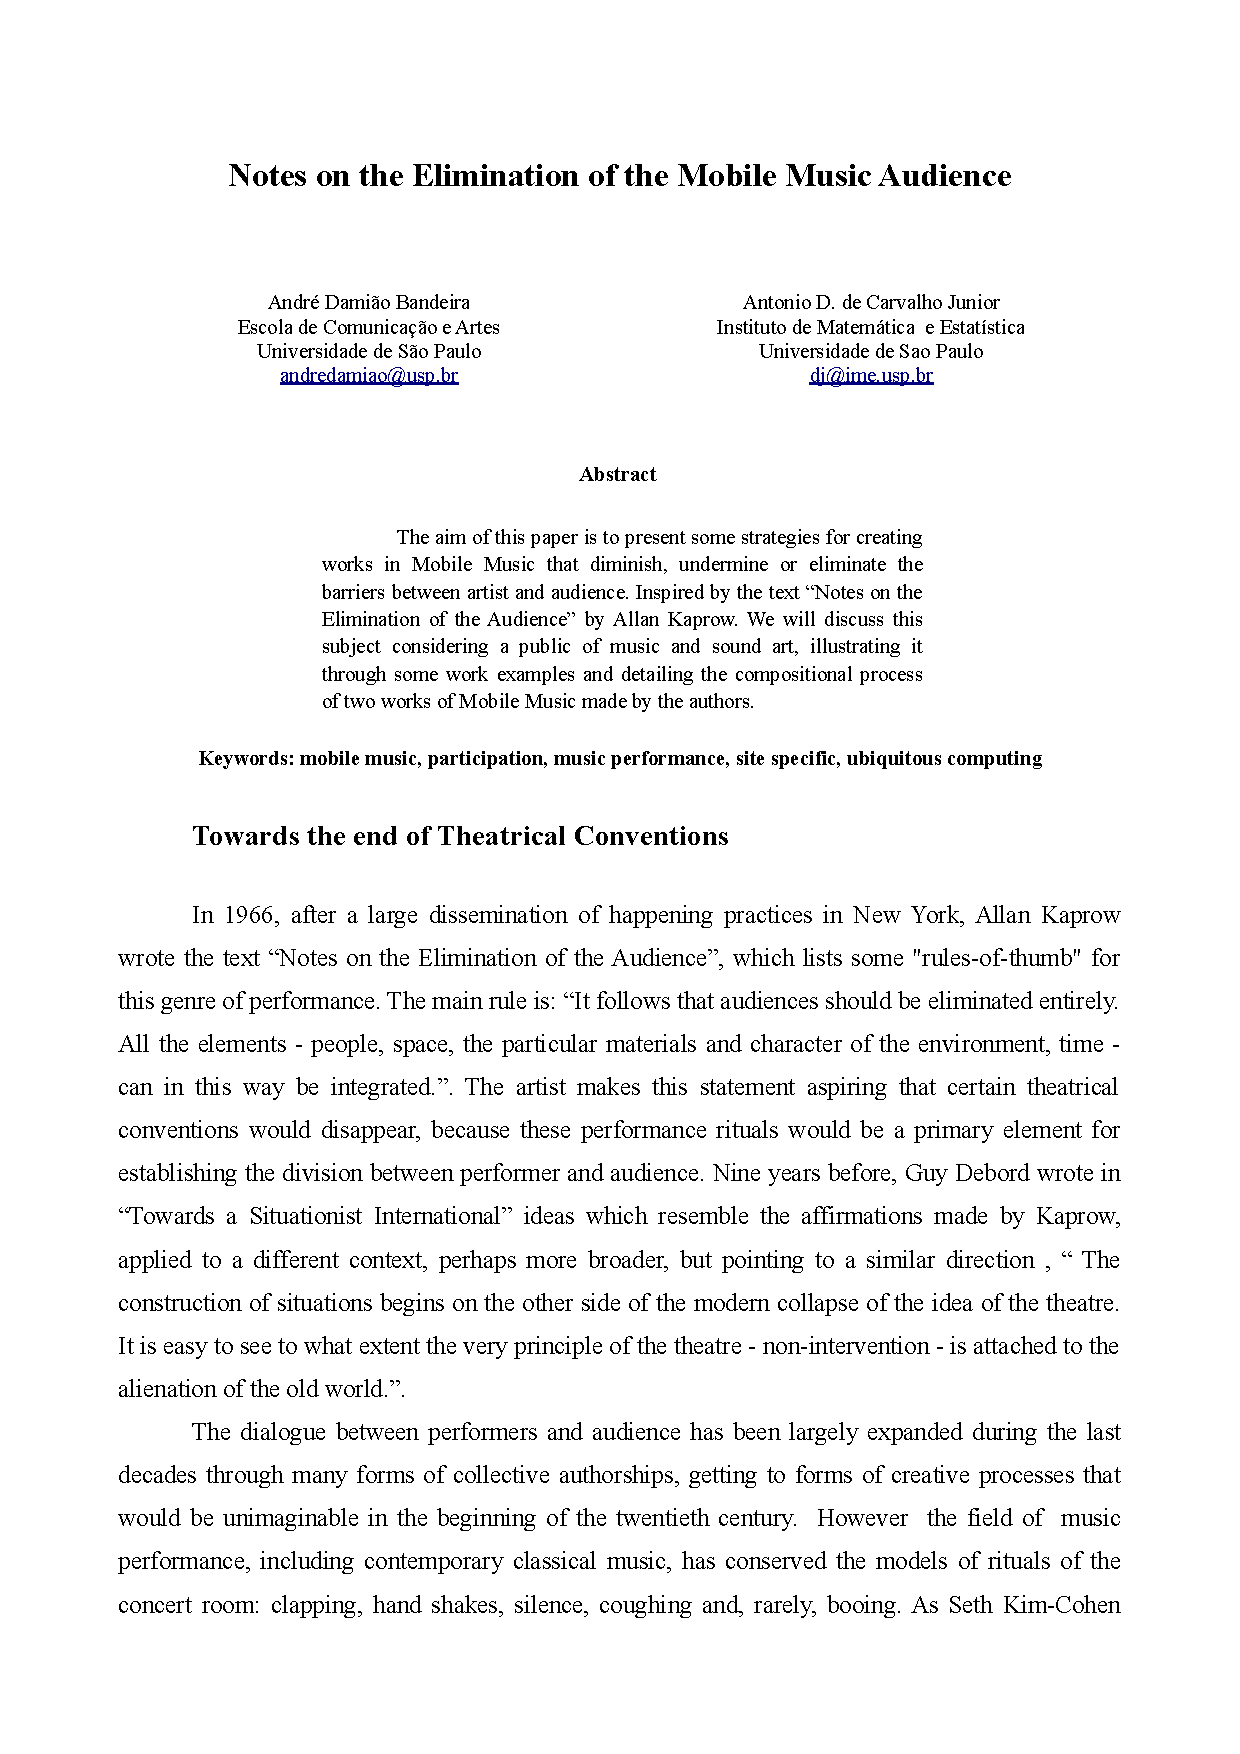
\includepdf[pages=-,frame,scale=0.8,pagecommand={}]{papers/2014-bienial-compressed.pdf}


%% ------------------------------------------------------------------------- %%
\section{ICMC 2014 - Sensors2PD: Mobile sensors and WiFi information as input for Pure Data}
\label{ape:papericmc2014}

\subsection*{Paper details}

Title: \textit{Sensors2PD: Mobile sensors and WiFi information as input for Pure Data}

Authors: Antonio Deusany de Carvalho Junior

\subsection*{Conference details}

Title: 40th International Computer Music Conference and 11th Sound and Music Computing Conference

Venue: Athens, Greece

Dates: September 14 to 20, 2014 

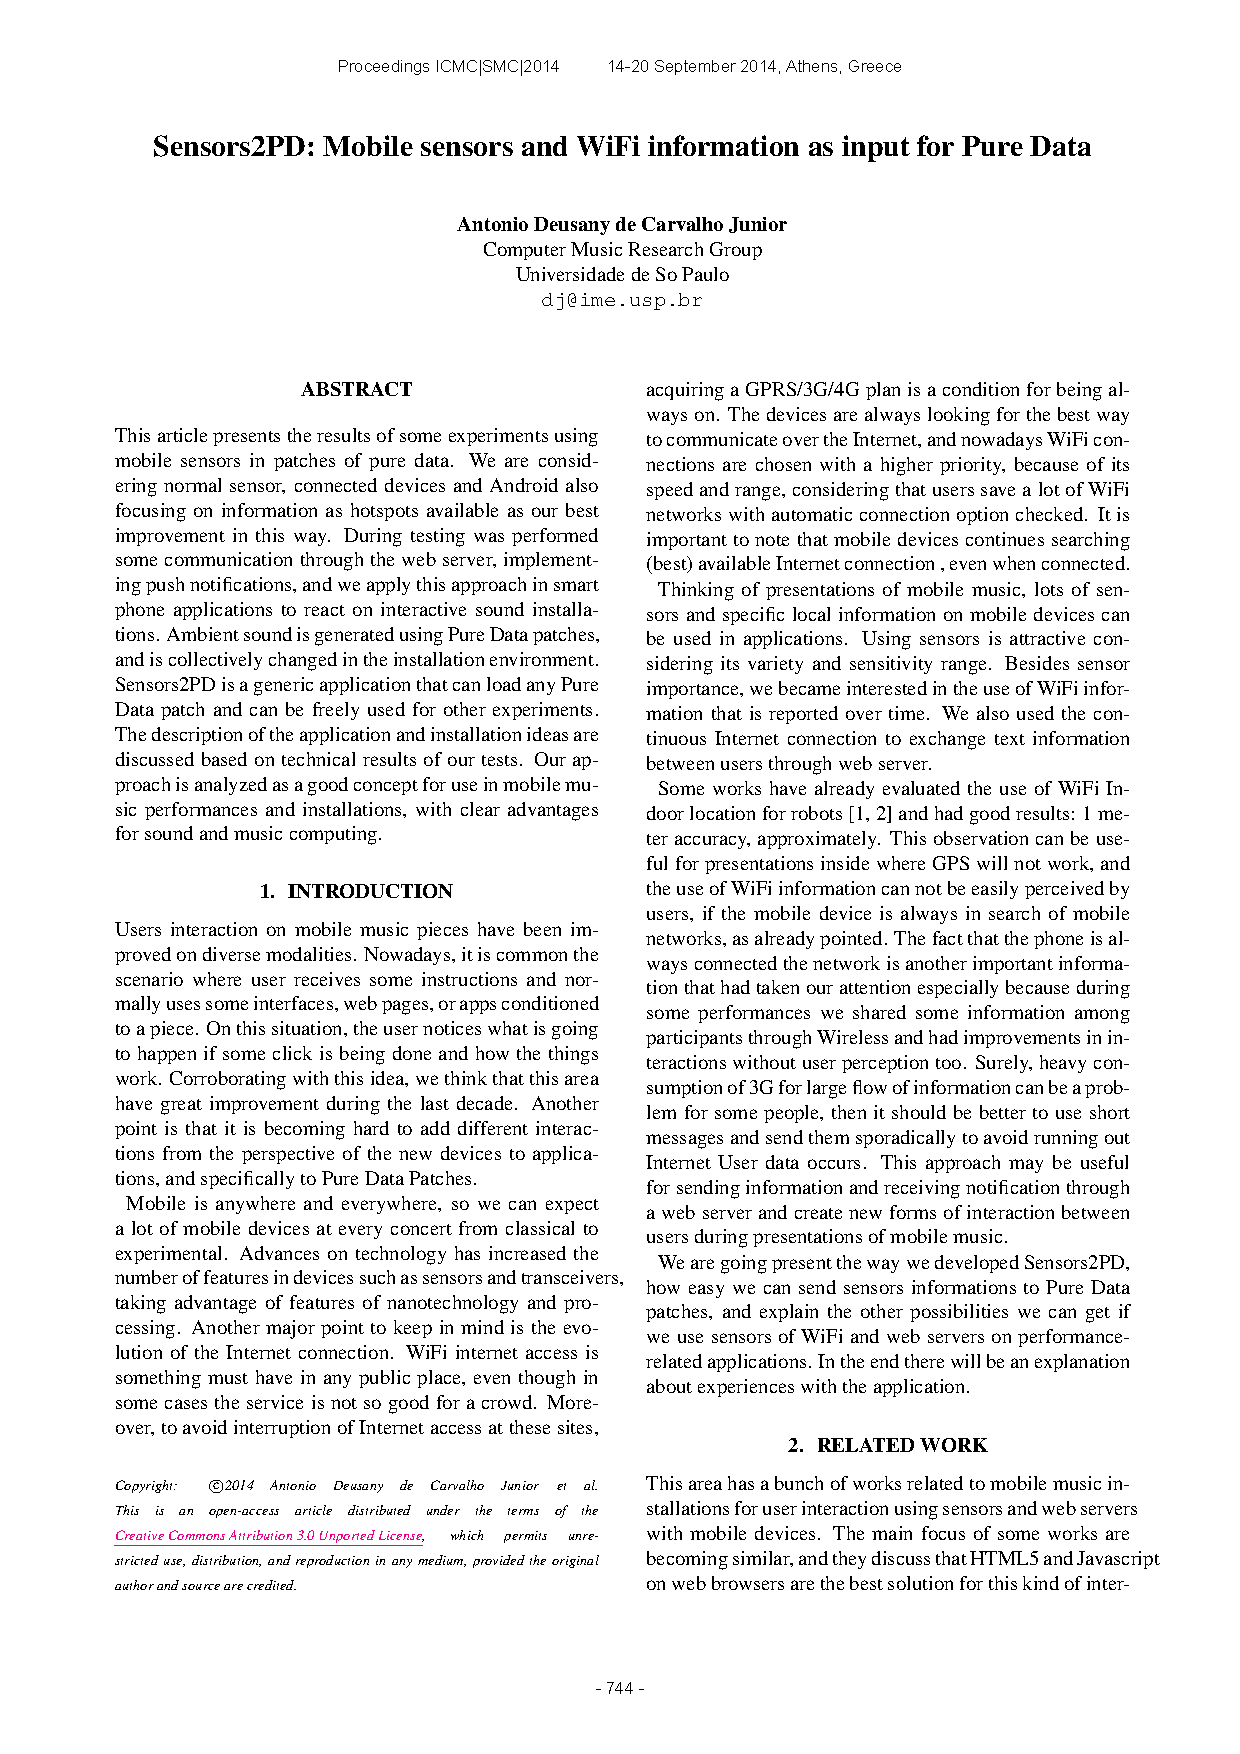
\includepdf[pages=-,frame,scale=0.8,pagecommand={}]{papers/2014-icmcsmc.pdf}

%% ------------------------------------------------------------------------- %%
\section{NIME 2015 - Indoor localization during installations using Wi-Fi}
\label{ape:papernime2015}

\subsection*{Paper details}

Title: \textit{Indoor localization during installations using Wi-Fi}

Authors: Antonio Deusany de Carvalho Junior

\subsection*{Conference details}

Title: 15th International Conference on New Interfaces for Musical Expression

Venue: Lousiana State University, Banton Rouge, LA, USA

Dates: May 31 to June 3, 2015

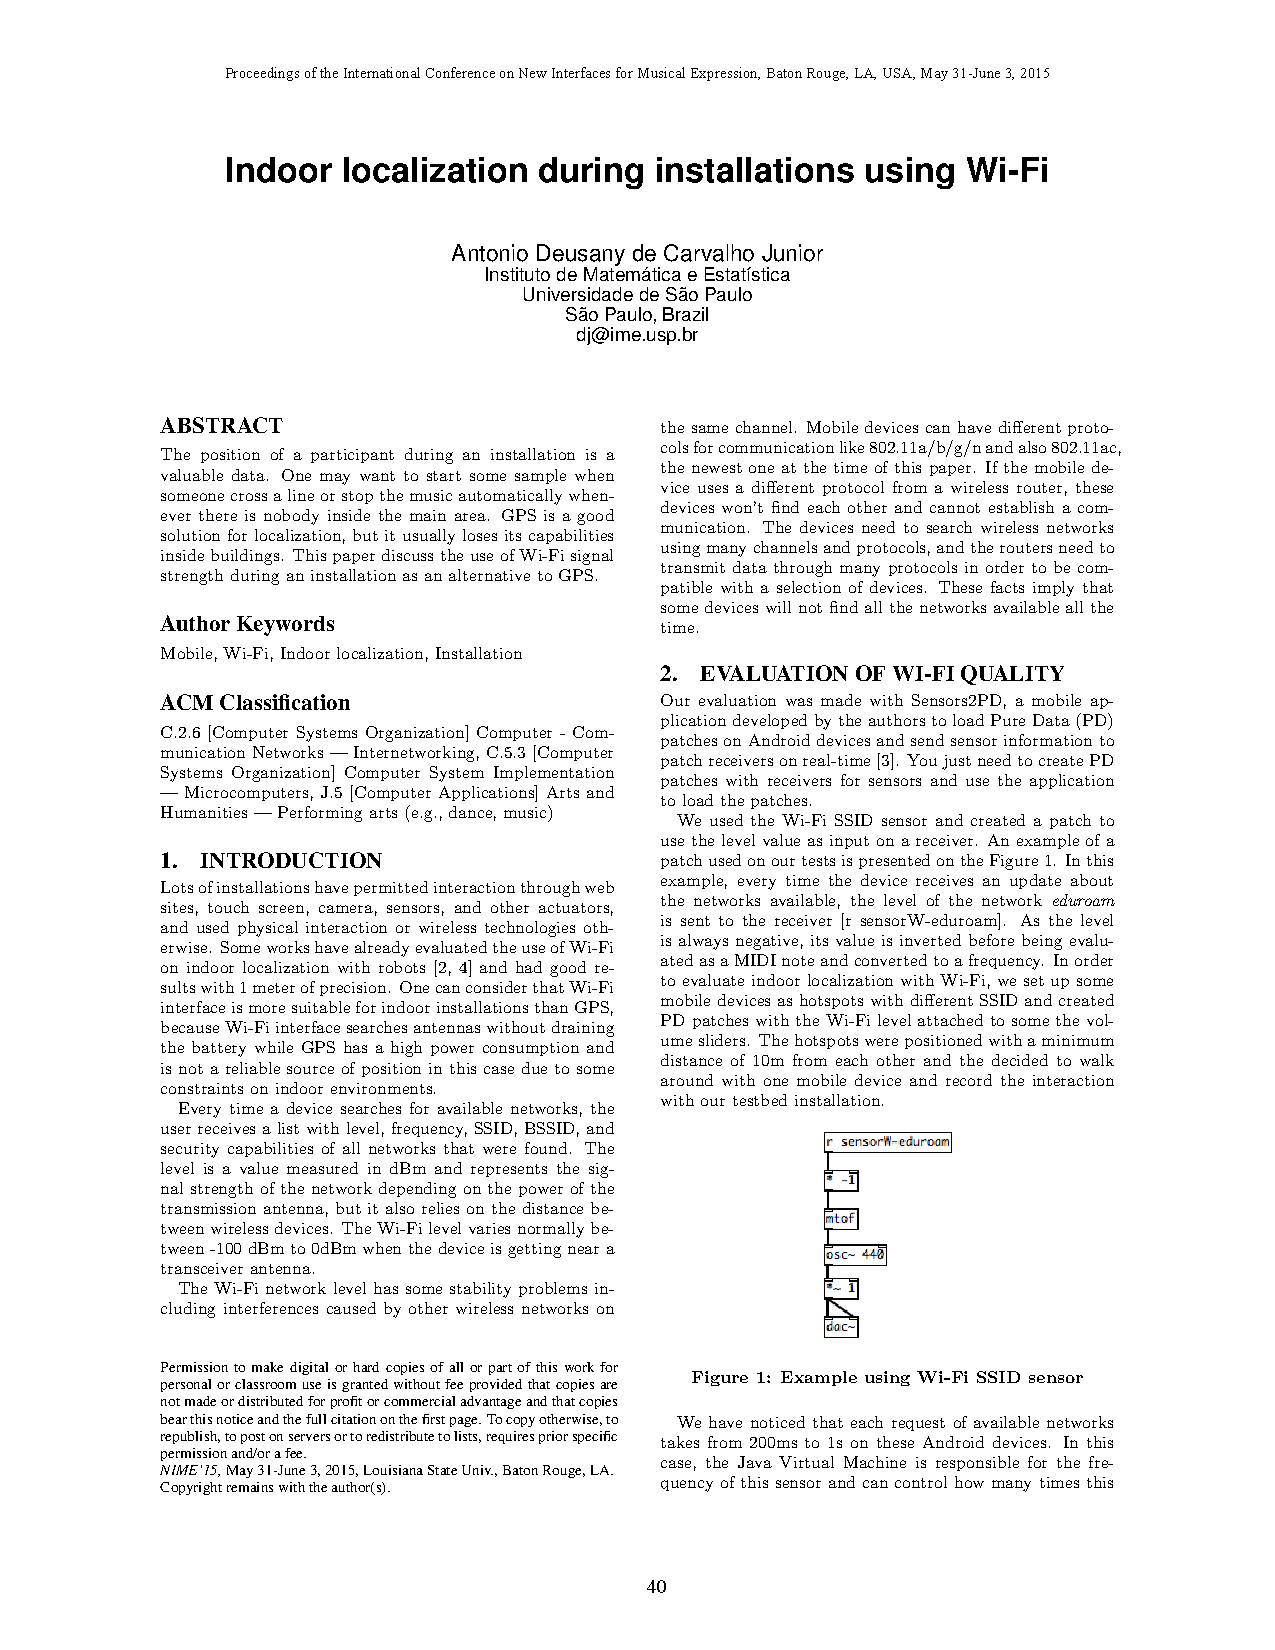
\includepdf[pages=-,frame,scale=0.8,pagecommand={}]{papers/2015-nime.pdf}

%% ------------------------------------------------------------------------- %%
\section{SMC 2015 - Sensors2OSC}
\label{ape:papersmc2015}

\subsection*{Paper details}

Title: \textit{Sensors2OSC}

Authors: Antonio Deusany de Carvalho Junior, Thomas Mayer

\subsection*{Conference details}

Title: 12th Sound and Music Computing Conference

Venue: Maynooth University, Ireland

Dates: July 26 to August 1, 2015

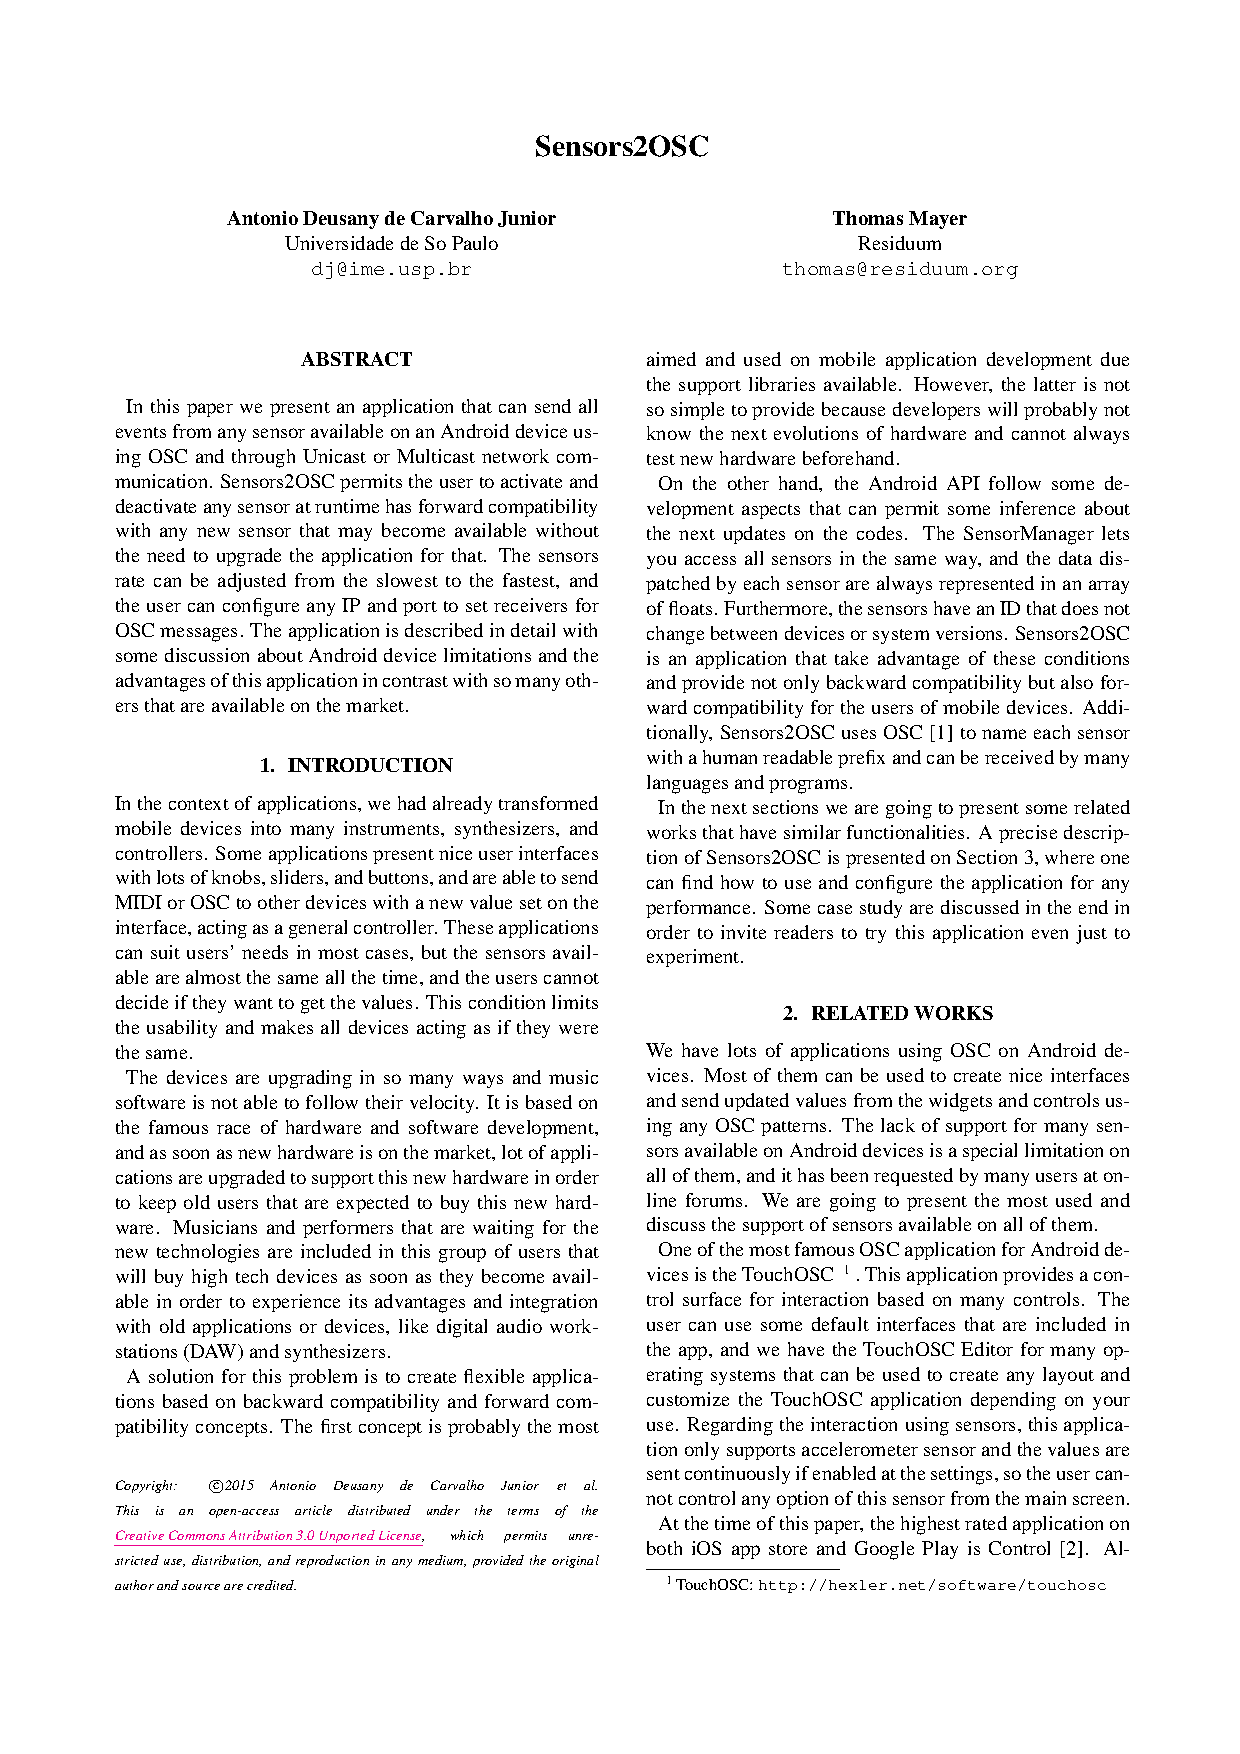
\includepdf[pages=-,frame,scale=0.8,pagecommand={}]{papers/2015-smc.pdf}


%% ------------------------------------------------------------------------- %%
\section{ICMC 2015 - Computer Music through the Cloud: Evaluating a Cloud Service for Collaborative Computer Music Applications}
\label{ape:papericmc2015}

\subsection*{Paper details}

Title: \textit{Computer Music through the Cloud: Evaluating a Cloud Service for Collaborative Computer Music Applications}

Authors: Antonio Deusany de Carvalho Junior, Marcelo Queiroz, Georg Essl

\subsection*{Conference details}

Title: 41st International Computer Music Conference~(ICMC)

Venue: University of North Texas, Denton, TX, USA

Dates: September 25 to October 1, 2015

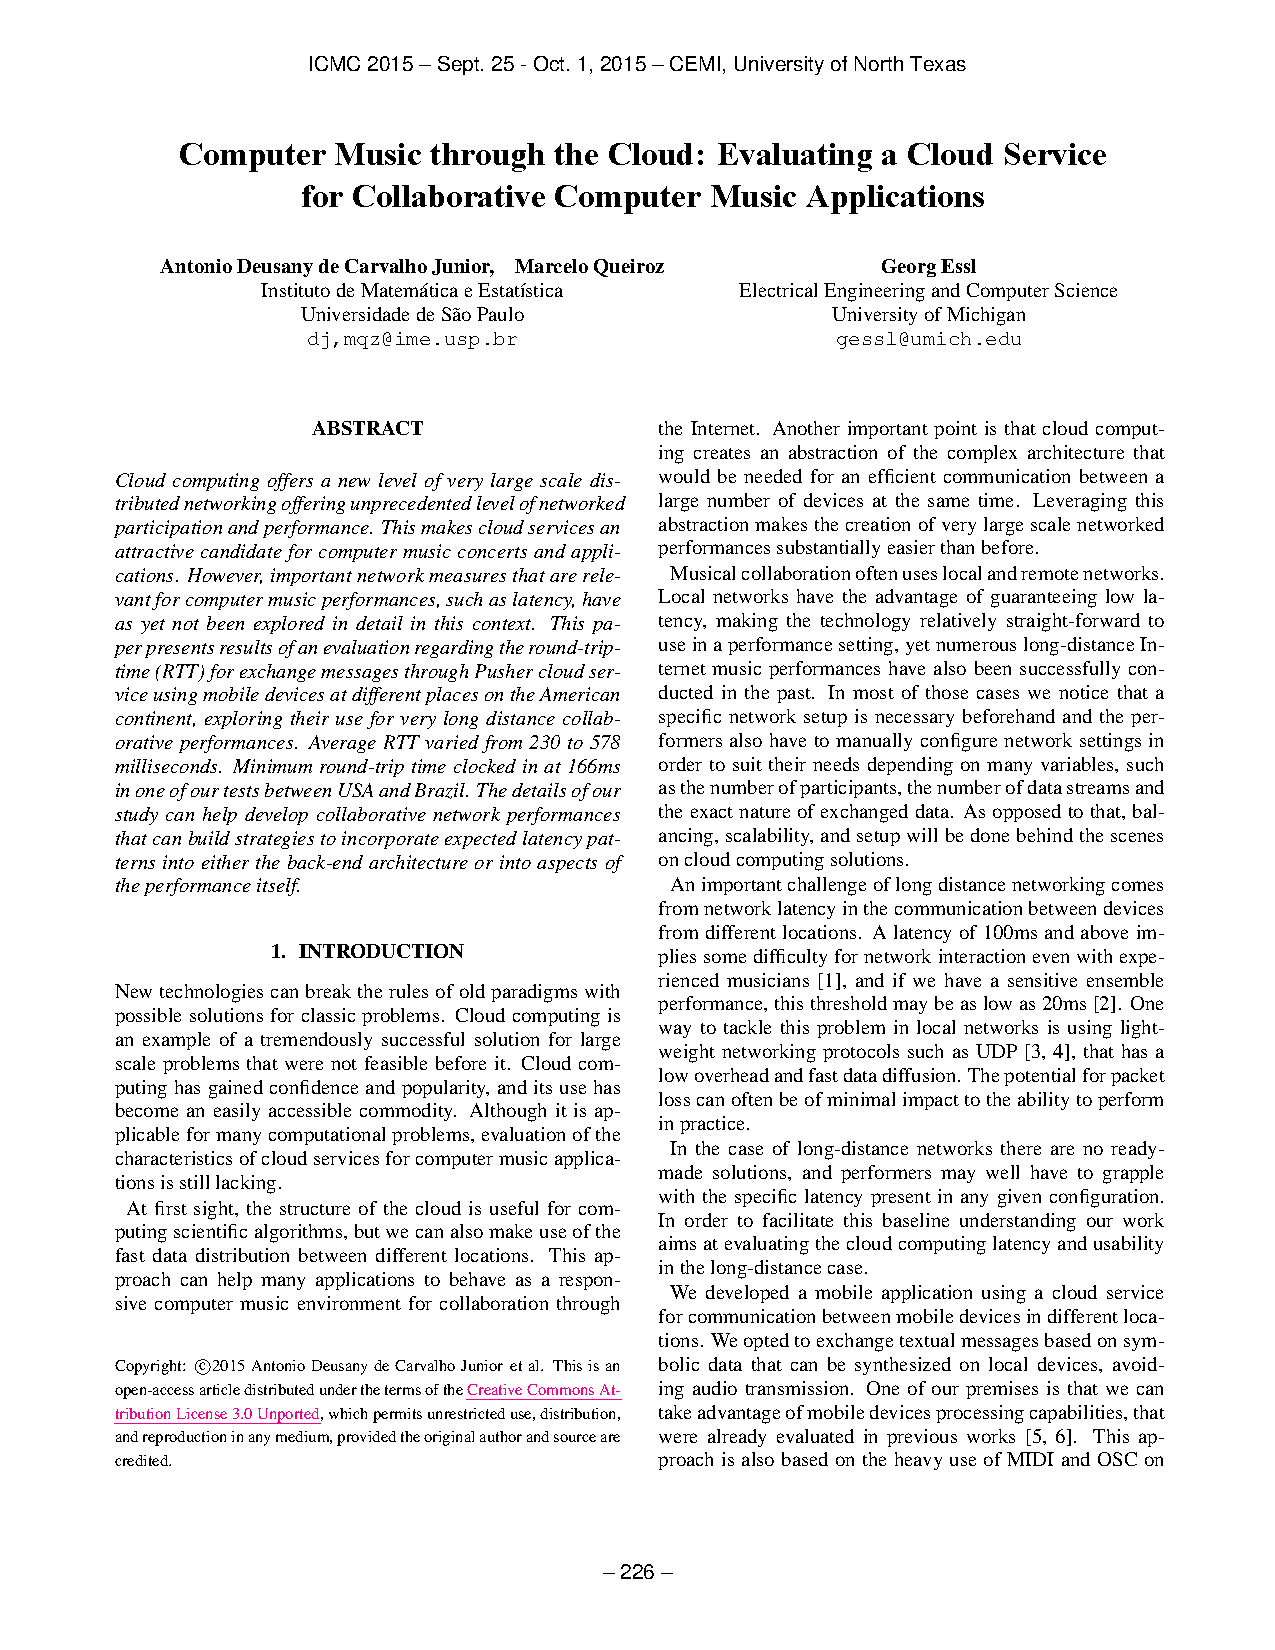
\includepdf[pages=-,frame,scale=0.8,pagecommand={}]{papers/2015-icmc.pdf}

%% ------------------------------------------------------------------------- %%
\section{ICLC 2015 - SuperCopair: Collaborative Live Coding on SuperCollider through the cloud}
\label{ape:papericlc2015}

\subsection*{Paper details}

Title: \textit{SuperCopair: Collaborative Live Coding on SuperCollider through the cloud}

Authors: Antonio Deusany de Carvalho Junior, Sang Won Lee, Georg Essl

\subsection*{Conference details}

Title: International Conference on Live Coding~(ICLC)

Venue: School of Music, University of Leeds, UK

Dates: July 13 to 15, 2015

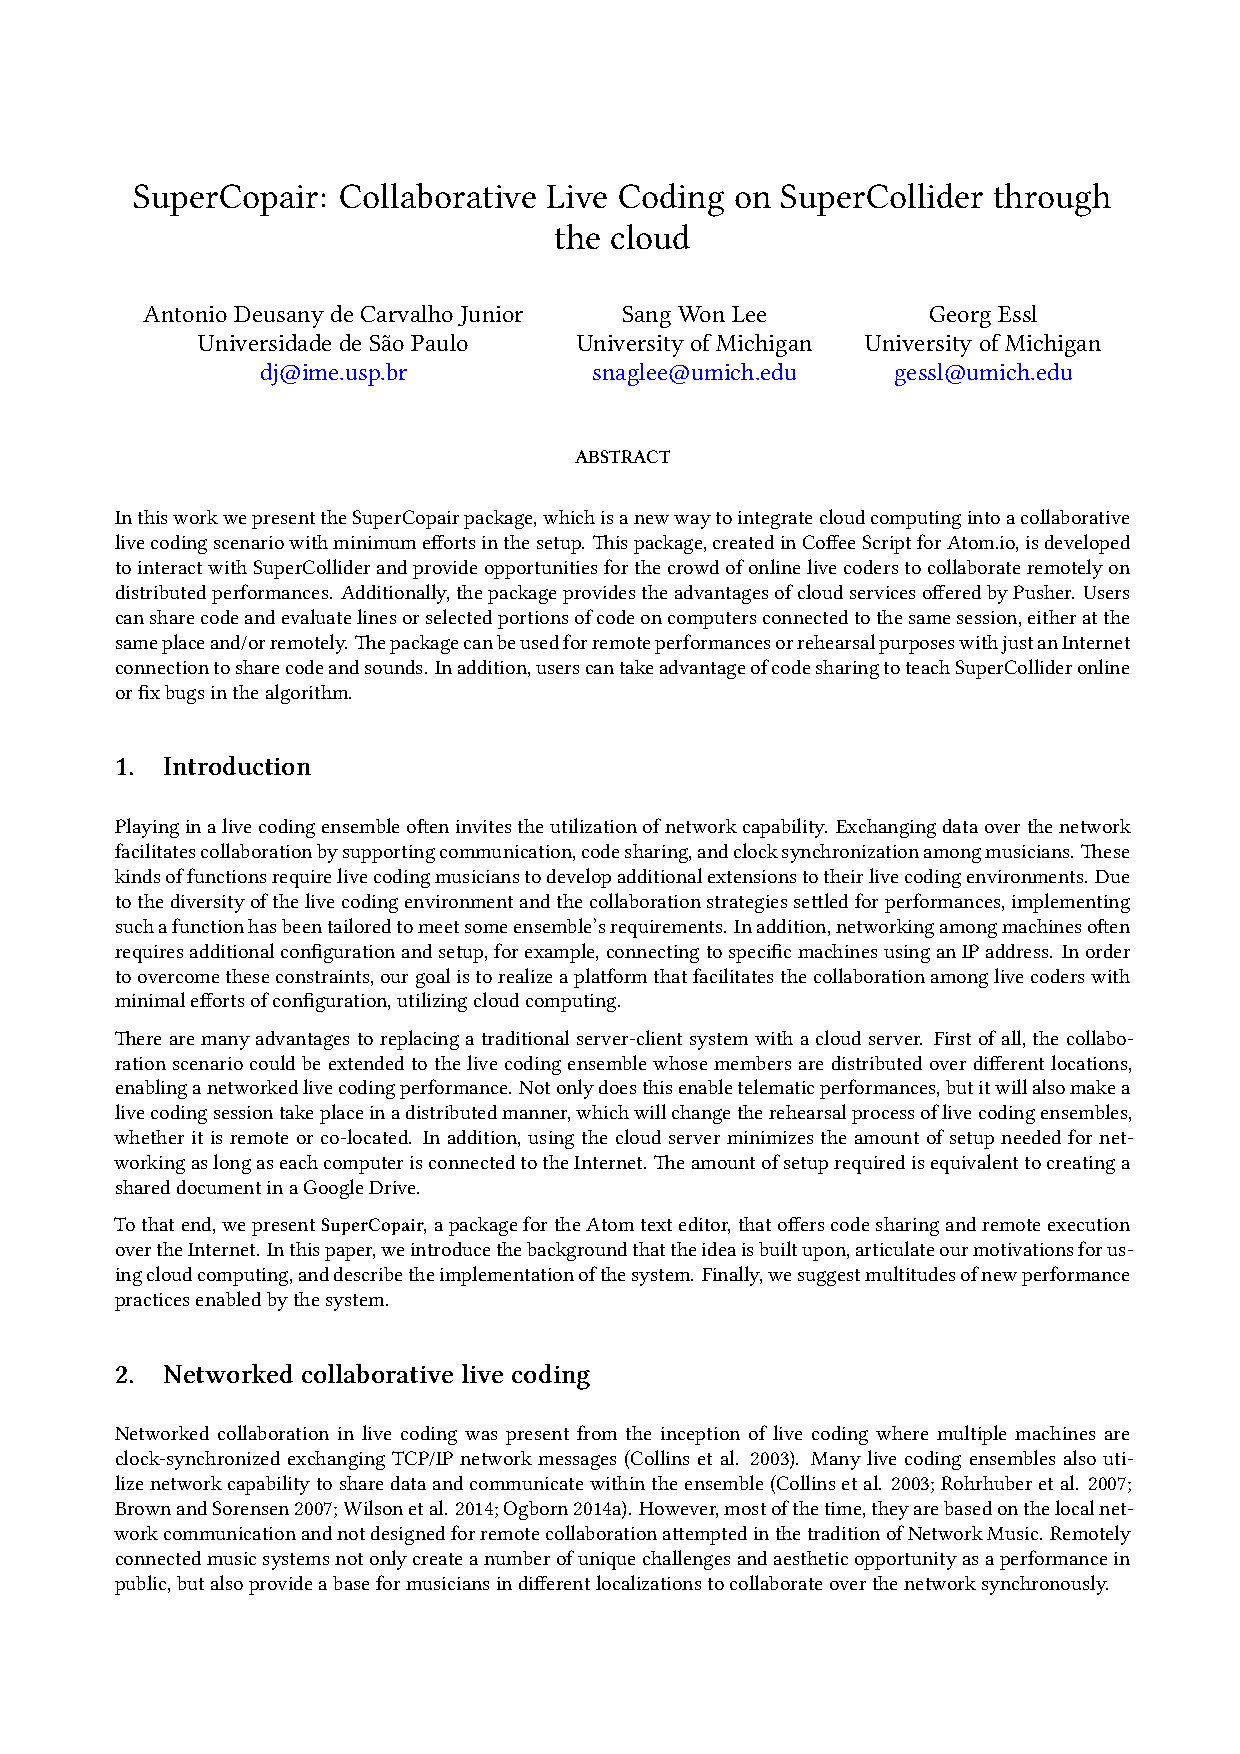
\includepdf[pages=-,frame,scale=0.8,pagecommand={}]{papers/2015-iclc.pdf}

%% ------------------------------------------------------------------------- %%
\section{CLEI 2015 - Cooperative Live Coding as an instructional model}
\label{ape:paperclei2015}

\subsection*{Paper details}

Title: \textit{Cooperative Live Coding as an instructional model}

Authors: Antonio Deusany de Carvalho Junior

\subsection*{Conference details}

Title: XLI Conferencia Latinoamericana en Informática~(CLEI)

Venue: Arequipa, Peru

Dates: October 19 to 23, 2015

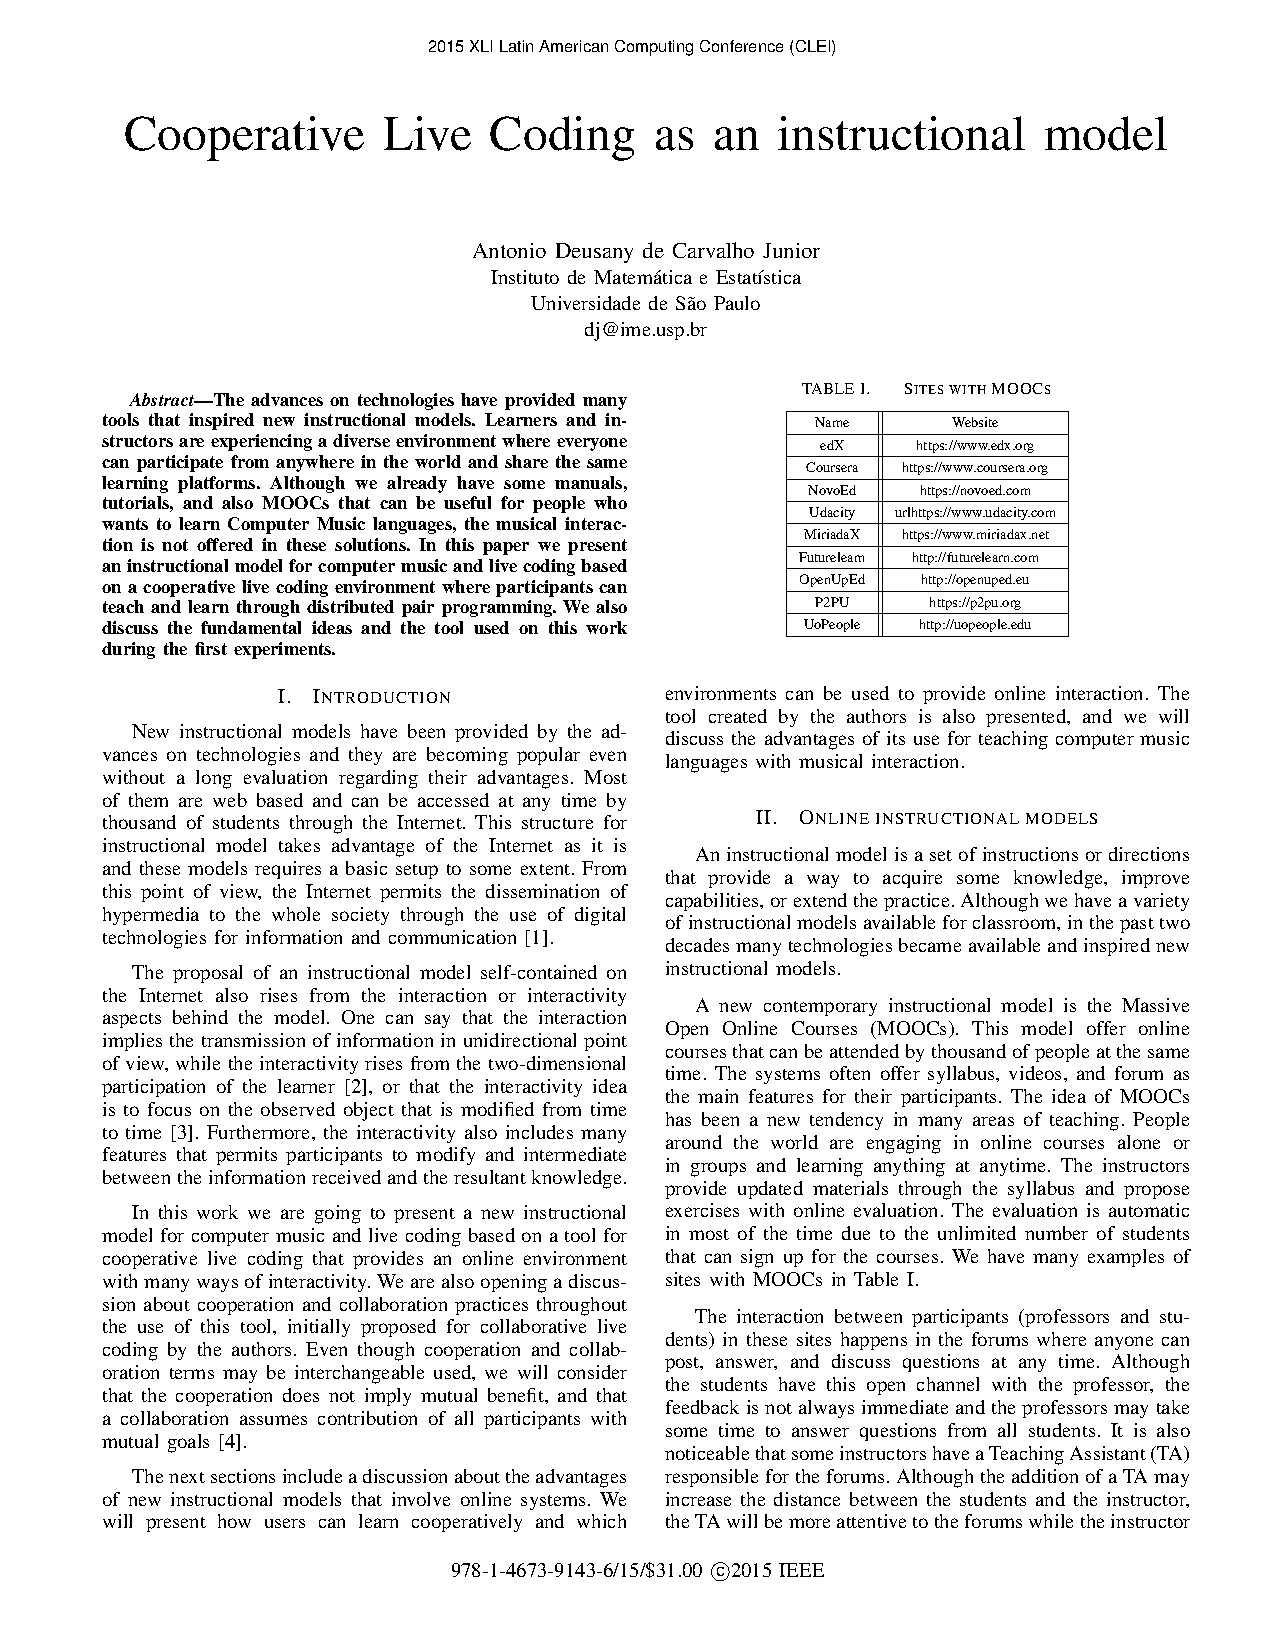
\includepdf[pages=-,frame,scale=0.8,pagecommand={}]{papers/2015-clei.pdf}


%% ------------------------------------------------------------------------- %%
\section{WAC 2016 - Crowd in C[loud]: Audience Participation Music with Online Dating Metaphor using Cloud Service}
\label{ape:paperwac2016}

\subsection*{Paper details}

Title: \textit{Crowd in C[loud]: Audience Participation Music with Online Dating Metaphor using Cloud Service}

Authors: Sang Won Lee, Antonio Deusany de Carvalho Junior, Georg Essl

\subsection*{Conference details}

Title: 2nd Web Audio Conference~(WAC)

Venue: Georgia Tech, Atlanta, GA, USA

Dates: April 4 to 6, 2016

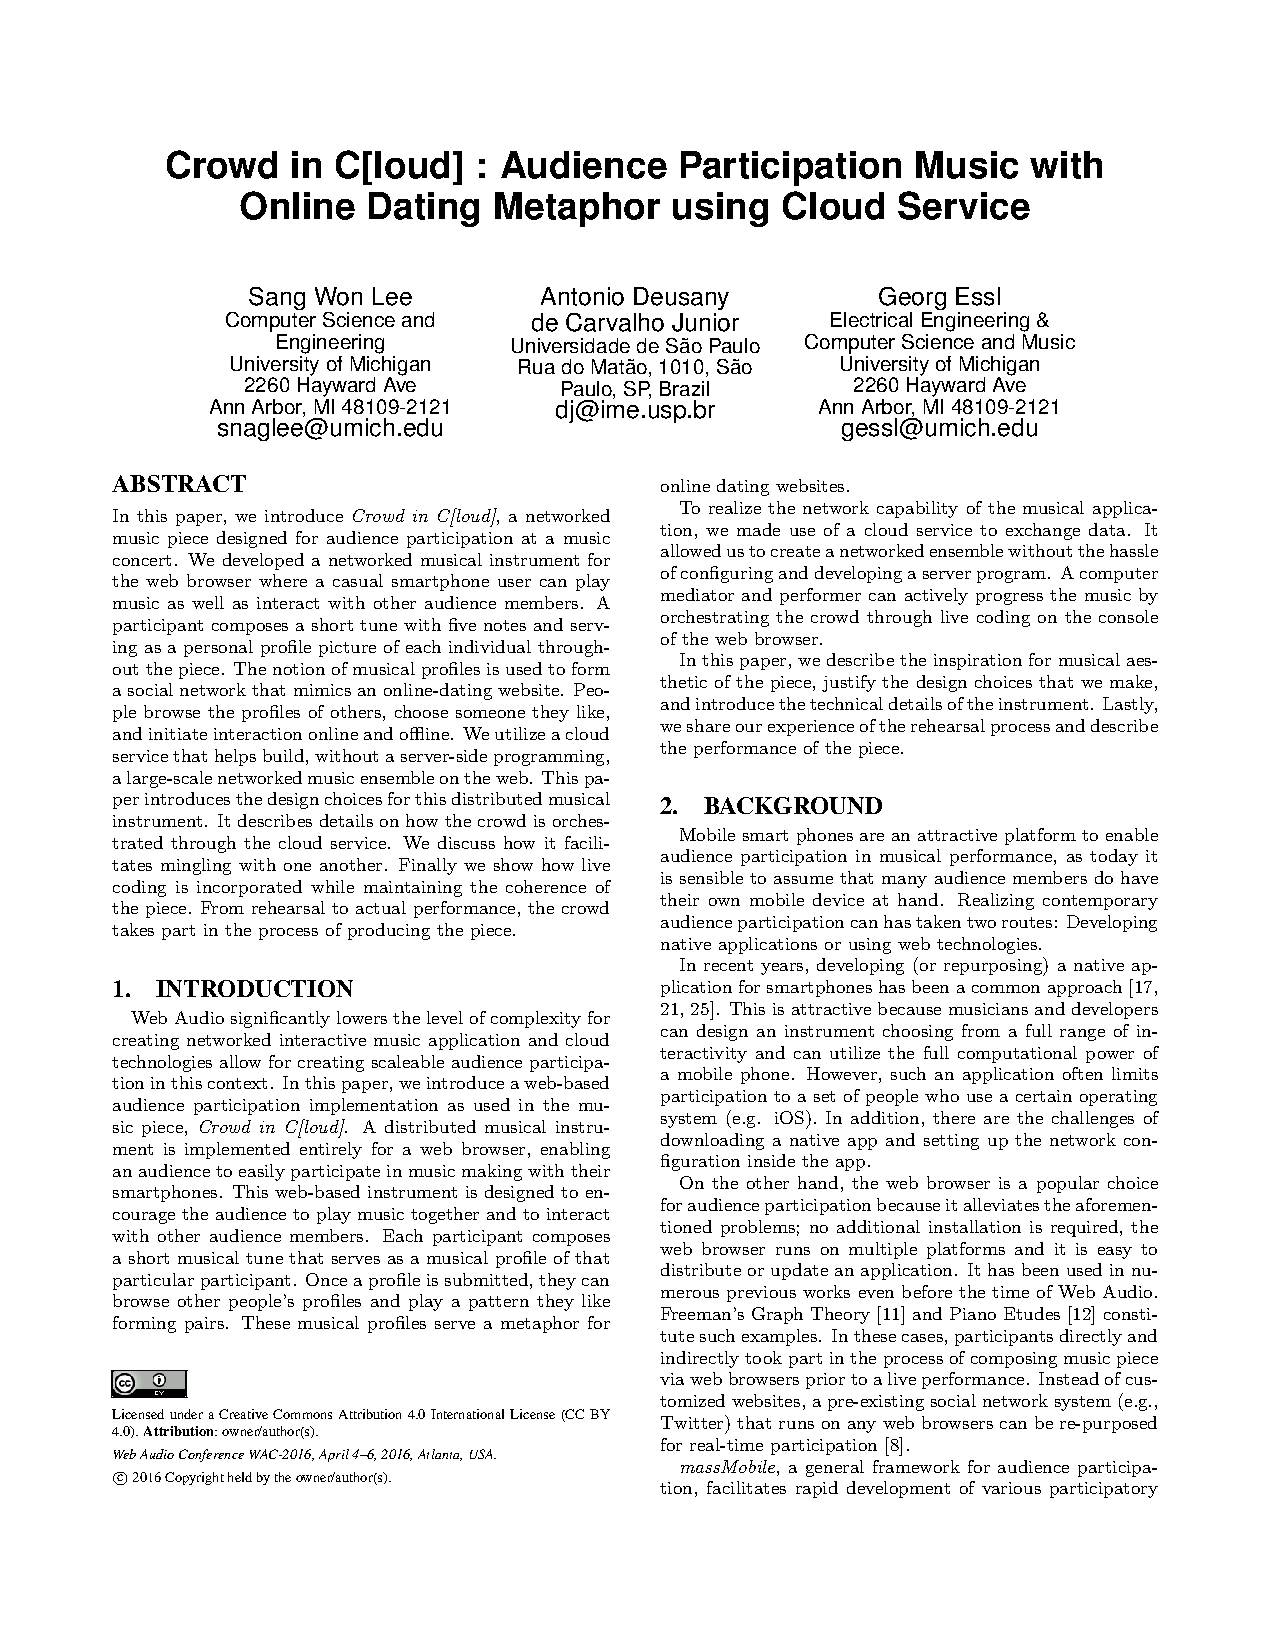
\includepdf[pages=-,frame,scale=0.8,pagecommand={}]{papers/2016-webaudio.pdf}


%% ------------------------------------------------------------------------- %%
\section{NIME 2016 - Understanding Cloud Service in the Audience Music Performance of Crowd in C[loud]}
\label{ape:papernime2016}

\subsection*{Paper details}

Title: \textit{Understanding Cloud Service in the Audience Music Performance of Crowd in C[loud]}

Authors: Antonio Deusany de Carvalho Junior, Sang Won Lee, Georg Essl

\subsection*{Conference details}

Title: 16th International Conference on New Interfaces for Musical Expression

Venue: Griffith University, Brisbane, Australia

Dates: July 11 to 15, 2016

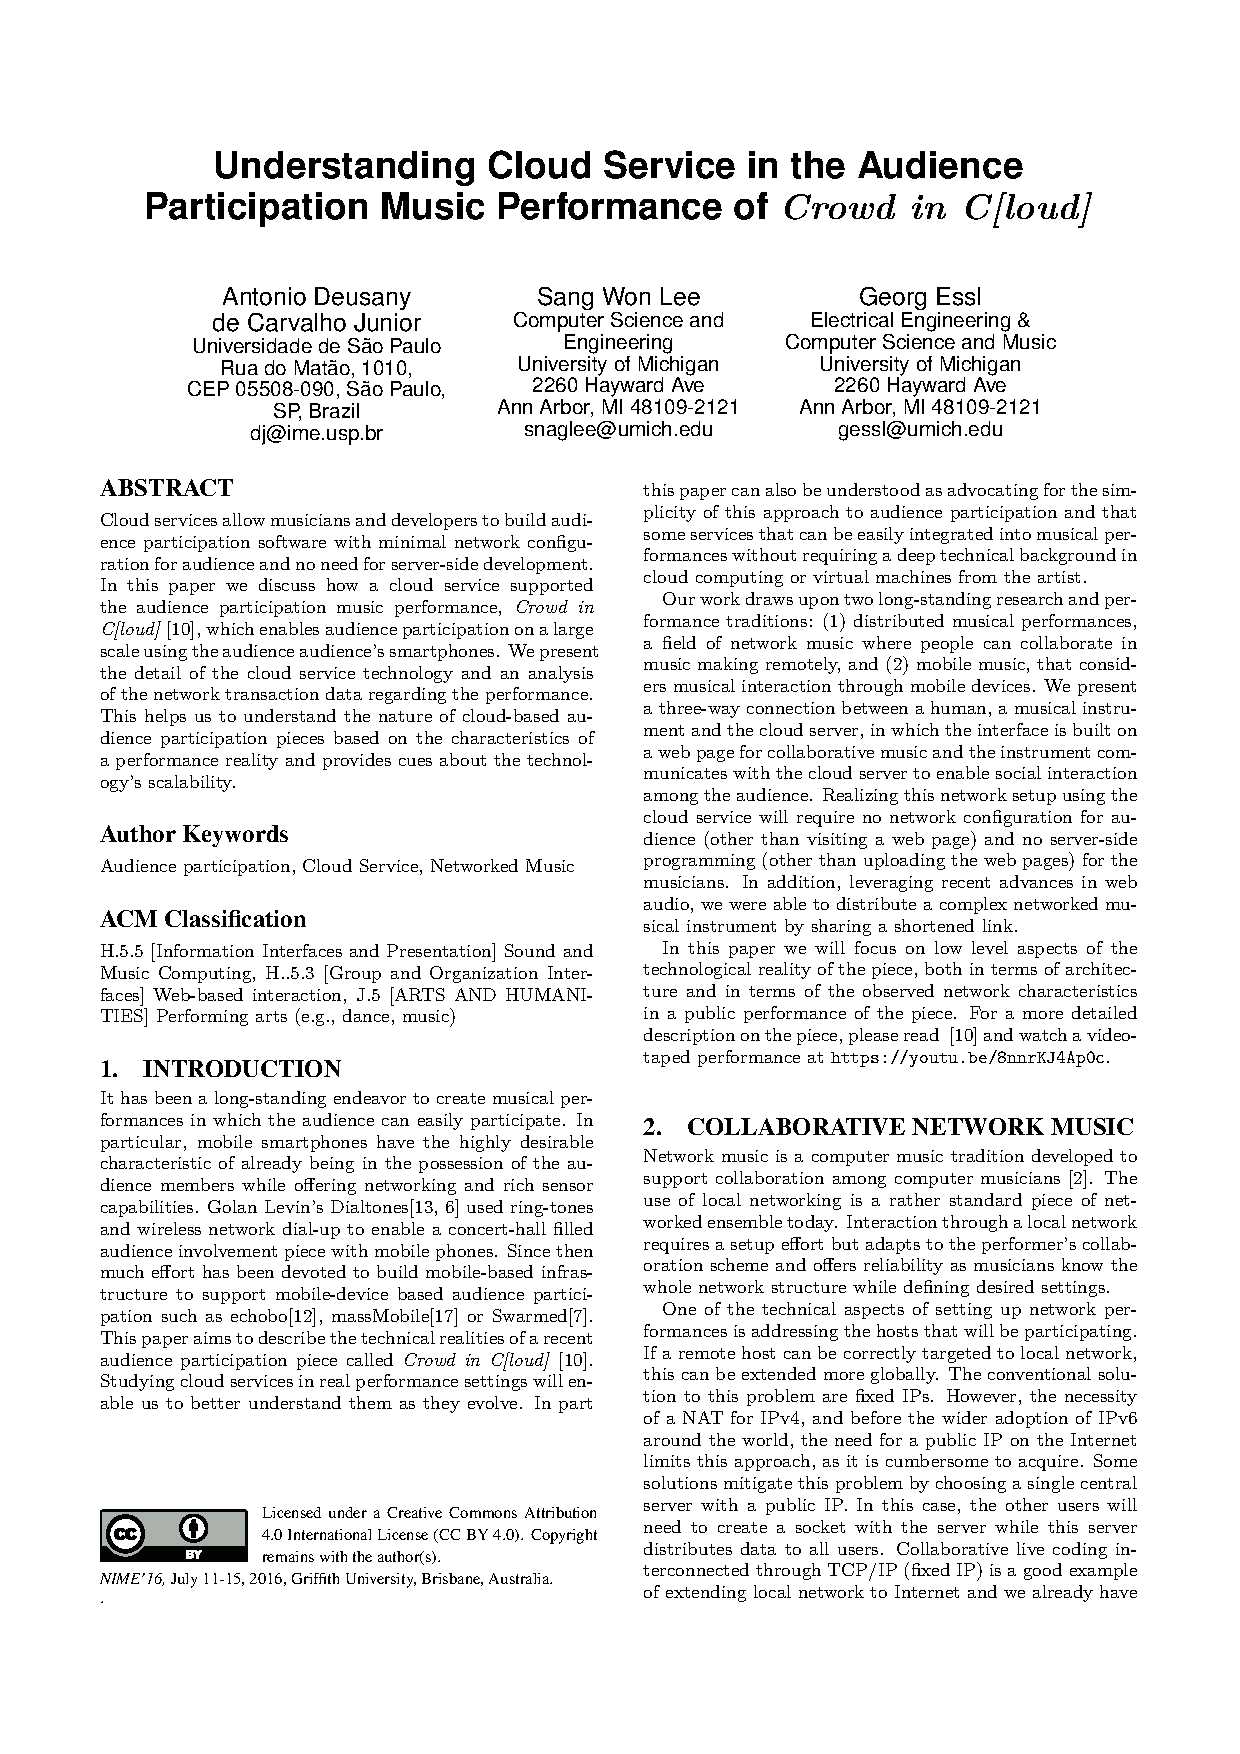
\includepdf[pages=-,frame,scale=0.8,pagecommand={}]{papers/2016-nime.pdf}

%% ------------------------------------------------------------------------- %%
\section{WAC 2017 - Open band: Audience Creative Participation Using Audio Synthesis}
\label{ape:paperwac2017}

\subsection*{Paper details}

Title: \textit{Open band: Audience Creative Participation Using Audio Synthesis}

Authors: Ariane Stolfi, Fábio Goródscy, Antonio Deusany de Carvalho Junior, Fernando Iazzetta, Mathieu Barthet

\subsection*{Conference details}

Title: 3rd Web Audio Conference~(WAC)

Venue: Centre for Digital Music, Queen Mary University of London, London, UK

Dates: August 21 to 23, 2017

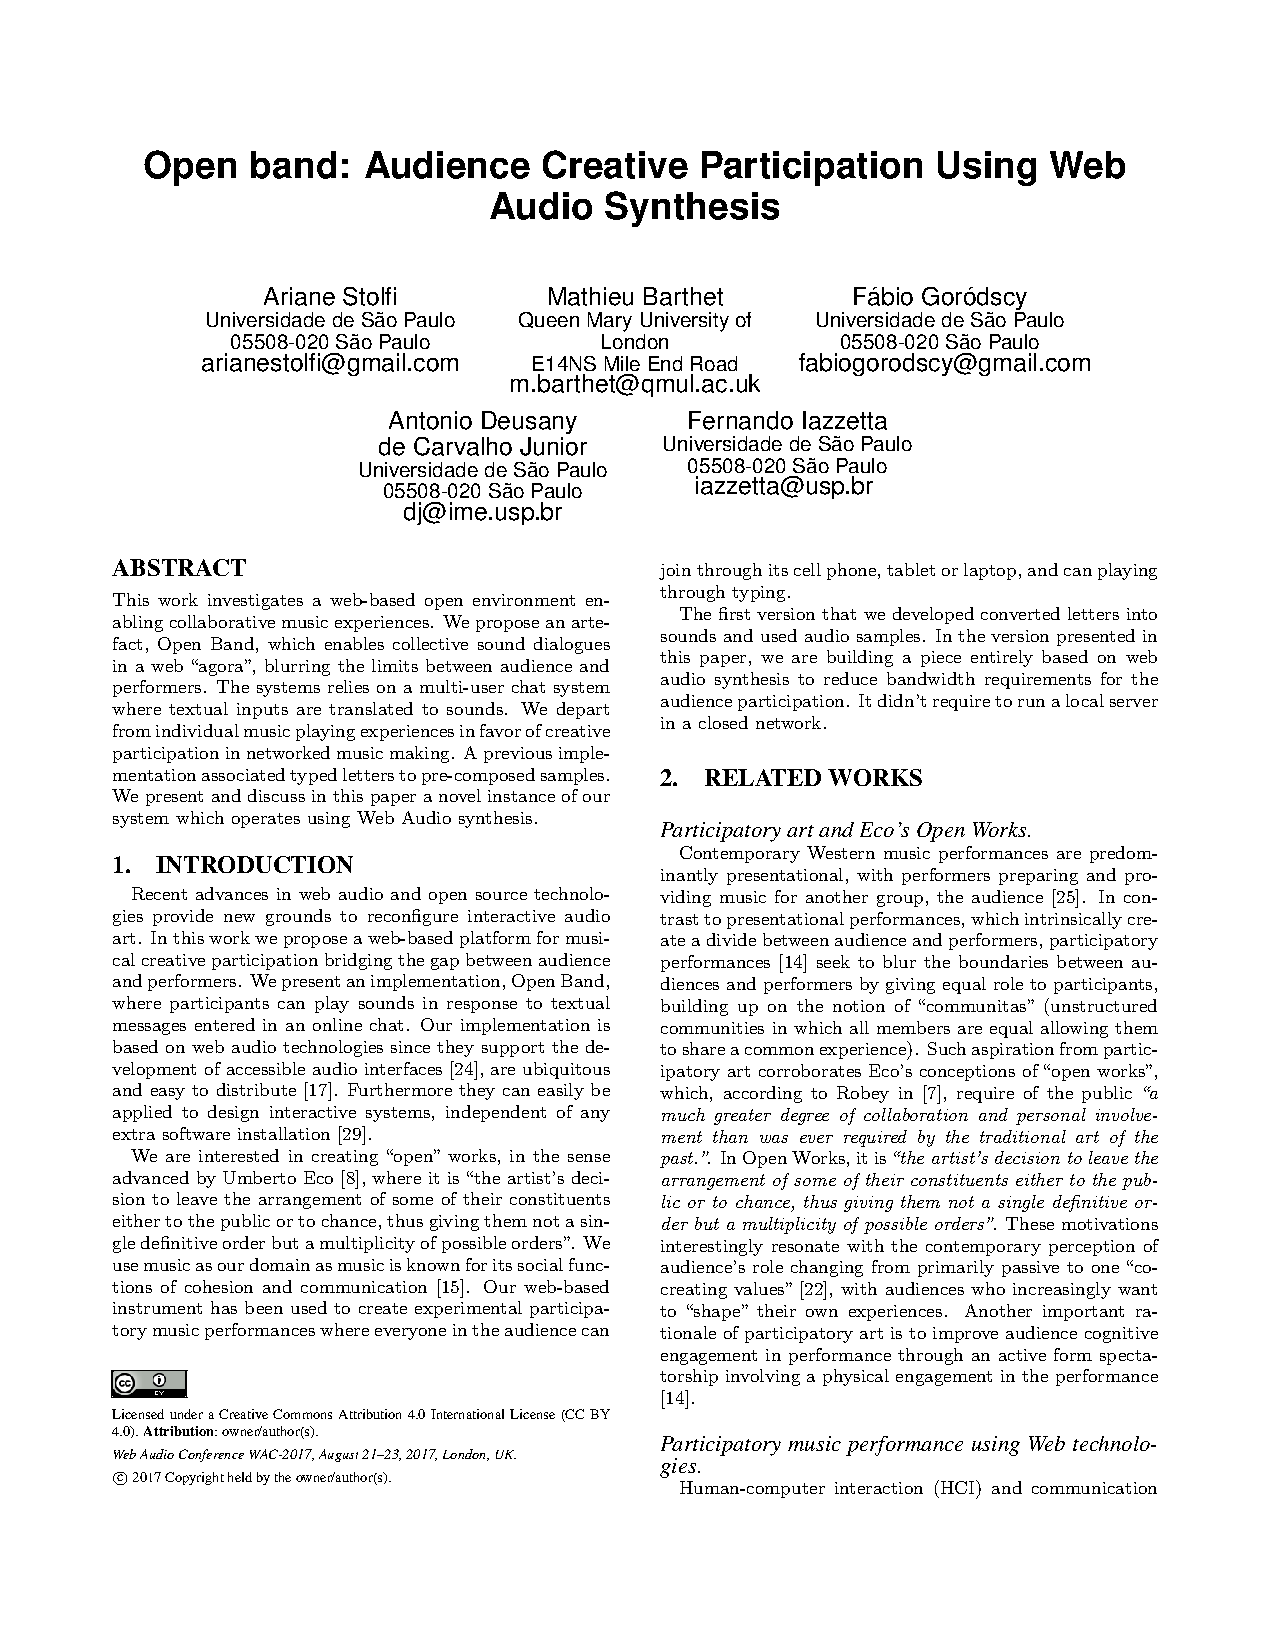
\includepdf[pages=-,frame,scale=0.8,pagecommand={}]{papers/2017-webaudio.pdf}

%% ------------------------------------------------------------------------- %%
\section{Audio Mostly 2017 - Open Band: A Platform for Collective Sound Dialogues}
\label{ape:paperam2017}

\subsection*{Paper details}

Title: \textit{Open band: A Platform for Collective Sound Dialogues}

Authors: Ariane Stolfi, Fábio Goródscy, Antonio Deusany de Carvalho Junior, Mathieu Barthet

\subsection*{Conference details}

Title: Audio Mostly

Venue: Centre for Digital Music, Queen Mary University of London, London, UK
 
Dates: August 23 to 25, 2017

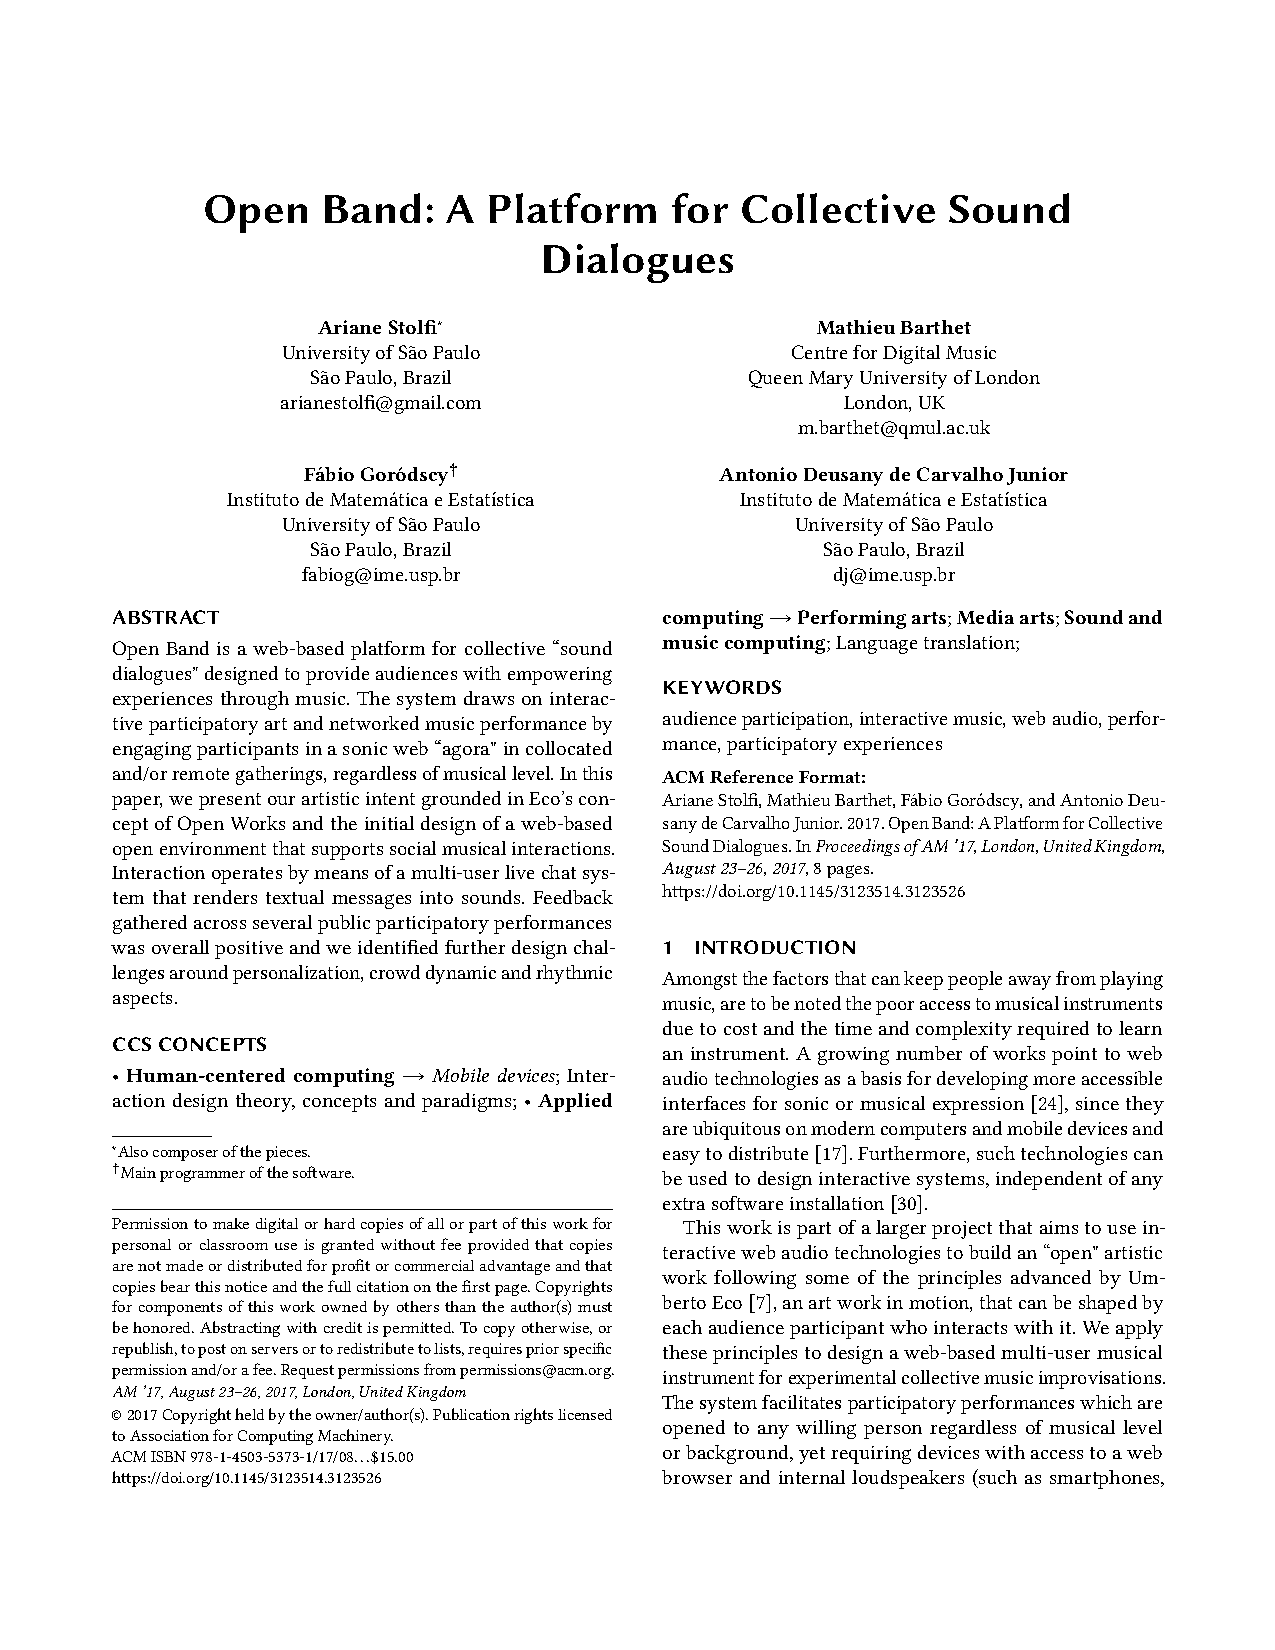
\includepdf[pages=-,frame,scale=0.8,pagecommand={}]{papers/2017-audiomostly.pdf}
